\documentclass[git,signature]{deltares_manual}

\svnid{$Id$}

\usepackage{hyperref}
\usepackage{listings}

\usepackage{lscape}
\usepackage{amssymb}
\usepackage{hyperref}
\usepackage{xcolor}

\begin{document}
\pagestyle{empty}
\renewcommand\BackgroundPicChapter{
    \put(0,0){
    \parbox[b][\paperheight]{\paperwidth}{
        \vspace{4\baselineskip}
        \hspace{220mm}
        \includegraphics[width=20mm]{Probabilistic-library-BOI-RWS-strookje.jpg}
        \vfill
        }
    }
}

\definecolor{codegreen}{rgb}{0,0.6,0}
\definecolor{codegray}{rgb}{0.5,0.5,0.5}
\definecolor{codepurple}{rgb}{0.58,0,0.82}
\definecolor{backcolour}{rgb}{0.95,0.95,0.92}

\lstdefinestyle{mystyle}{
    backgroundcolor=\color{backcolour},
    commentstyle=\color{codegreen},
    keywordstyle=\color{blue},
    numberstyle=\tiny\color{codegray},
    stringstyle=\color{codepurple},
    basicstyle=\ttfamily\footnotesize,
    breakatwhitespace=false,
    breaklines=true,
    captionpos=b,
    keepspaces=true,
    numbers=left,
    numbersep=5pt,
    showspaces=false,
    showstringspaces=false,
    showtabs=false,
    tabsize=2
}

\renewcommand{\contactsalesandsupport}{
	\textbf{Contact:}\\
	\begin{tabular}[t]{@{}p{0.50\textwidth}p{0.50\textwidth}}
	\vspace*{-1.5\baselineskip}
	\begin{tabbing}
	Informatiepunt Leefomgeving  \\
	Rijkswaterstaat WVL \\
	P.O. 2232 \\
	3500 GE Utrecht \\
	The Netherlands \\
	\end{tabbing}
	&
	\vspace*{-1.5\baselineskip}
	\begin{tabbing}
	telephone: \= +31\,88\,797\,0790 \\
	www:       \> https://iplo.nl/ \\
	\end{tabbing}
	\end{tabular}
}

\lstset{style=mystyle}
\lstset{language=Fortran}

\newcommand{\hr}{Hydra-Ring\xspace} 
\newcommand{\probLib}{Probabilistic Library\xspace} 
\newcommand{\OET}{Open Earth Tools\xspace} 
\newcommand{\cmark}{\ding{51}}
\newcommand{\xmark}{\ding{55}}
\newcommand{\probLibVersion} {24.1.1}
\newcommand{\probLibProject}{11209269-008}
\newcommand{\datetests}{the 30$^{th}$ of January, 2024}

\client{Rijkswaterstaat}
\contact{--}
\documentid{--}
\disclaimer{--}
\projectnumber{\probLibProject{}}
\classification{--}
\references{--}
\date{\today}

\hyphenation{pro-ba-bi-lis-tische}
\hyphenation{be-schrijft}

\title{Probabilistic Library}
\subtitle{}
\manualtype{Functional Design}
\distribution{}
\contact{---}
\version{\probLibVersion{}}
\documentid{---}
\disclaimer{}
\pagestyle{empty}
\cleardoublepage
\pagestyle{empty}

\reference{11209269-008-GEO-0009}
\keywords{probabilistic library, WBI2023, BOI, functional design, (non-)functional requirements}
\summary{This document describes the \textit{Functional design} of the Probabilistic Library \textbf{version \probLibVersion{}}, part of BOI (in Dutch: \textit{Beoordelings- en Ontwerp Instrumentarium}). The BOI program derives guidelines, methods and tools for the statutory safety assessment and design of flood defences in the Netherlands. The Probabilistic Library provides a set of routines that enable system reliability analyses. The general goal of system reliability analyses is the derivation of the probability of failure of a system consisting of multiple components. The functional design describes functional and non-functional requirements imposed on the Probabilistic Library.}

%\versioni{1.0}
%\datei{Dec 2019}
%\authori{Karolina \newline Wojciechowska}
%\revieweri{Ferdinand \newline Diermanse \newline Tom The \newline Hans van Putten}
%\approvali{Jan Aart \newline van Twillert}
%
%\versionii{2.0}
%\dateii{Feb 2021}
%\authorii{Karolina \newline Wojciechowska}
%\reviewerii{Ferdinand \newline Diermanse \newline Rob Prevel}
%\approvalii{Jan Aart \newline van Twillert}
%
%\versioniii{3.0}
%\dateiii{May 2022}
%\authoriii{Karolina \newline Wojciechowska}
%\revieweriii{Ferdinand \newline Diermanse \newline Rob Prevel}
%\approvaliii{Jan Aart \newline van Twillert}

\versioni{4.0}
\datei{Juni 2023}
\authori{Karolina \newline Wojciechowska}
\revieweri{Arjen Markus \newline Marcel Pastoors}
\approvali{Jan Aart \newline van Twillert}

\status{Final}

\signatureGB

\pagestyle{empty}
\cleardoublepage
\pagestyle{empty}

\reference{11209269-008-GEO-0009}
\keywords{probabilistische bibliotheek, WBI2023, BOI, functioneel ontwerp, (niet-)functionele eisen}
\summary{Dit document beschrijft het \textit{Functioneel ontwerp} van de Probabilistische Bibliotheek \textbf{versie \probLibVersion{}}, onderdeel van BOI (Beoordelings- en Ontwerp Instrumentarium). Het BOI-programma bepaalt richtlijnen, methoden en instrumenten voor de wettelijke veiligheidsbeoordeling en ontwerpen van waterkeringen in Nederland. De probabilistische bibliotheek biedt een set routines, die analyses van de systeembetrouwbaarheid mogelijk maken. Het algemene doel van systeembetrouwbaarheidsanalyses is het afleiden van de faalkans van een systeem dat uit meerdere componenten bestaat. Het functionele ontwerp beschrijft functionele en niet-functionele eisen, die aan de Probabilistische Bibliotheek worden opgelegd.}

%\versioni{1.0}
%\datei{Dec 2019}
%\authori{Karolina \newline Wojciechowska}
%\revieweri{Ferdinand \newline Diermanse \newline Tom The \newline Hans van Putten}
%\approvali{Jan Aart \newline van Twillert}
%
%\versionii{2.0}
%\dateii{Feb 2021}
%\authorii{Karolina \newline Wojciechowska}
%\reviewerii{Ferdinand \newline Diermanse \newline Rob Prevel}
%\approvalii{Jan Aart \newline van Twillert}
%
%\versioniii{3.0}
%\dateiii{May 2022}
%\authoriii{Karolina \newline Wojciechowska}
%\revieweriii{Ferdinand \newline Diermanse \newline Rob Prevel}
%\approvaliii{Jan Aart \newline van Twillert}

\versioni{4.0}
\datei{June 2023}
\authori{Karolina \newline Wojciechowska}
\revieweri{Arjen Markus \newline Marcel Pastoors}
\approvali{Jan Aart \newline van Twillert}

\status{Definitief}

\signatureNL
\setgitdirectory{../.git}

\deltarestitle

\chapter{Introduction}
\section{Background}
The primary flood defences in the Netherlands are periodically assessed against the statutory safety standards, which are expressed in terms of maximum allowable flooding probabilities. The methods and (software) tools used in the assessment are prescribed by law and are part of the \textit{Wettelijk en BeoordelingsInstrumentarium} (WBI). The \textit{Beoordelings- en Ontwerp Instrumentarium} (BOI) derives guidelines, methods and tools for the safety assessment and design of flood defences.

As part of the BOI program, Deltares has developed a set of software tools consisting of:
\begin{itemize}
\item Riskeer: a user interface to facilitate the assessment process.
\item D-Soil model for the schematisation of the subsoil.
\item \hr: the probabilistic core of Riskeer.
\item Software library with failure mechanisms.
\item Software library with algorithms for system reliability analyses (i.e. the \probLib).
\item Basic modules around a number of failure mechanisms.
\end{itemize}

\hr is the probabilistic core of Riskeer and it is used to compute the failure probability of a flood defence system composed of a number of dike segments, dune segments and hydraulic structures. For that purpose, \hr makes use of the \probLib that provides a set of algorithms for system reliability analysis. The general goal of system reliability analysis is the derivation of the probability of failure of a system consisting of multiple components.

Until 2019, the \probLib was part of \hr. In order to enable system reliability analysis for other software applications, the \probLib has been separated from \hr. The various software components and the relations between them are presented in \Fref{fig_BOI}.

\begin{figure}[H]\centering
\includegraphics*[width=6in, height=6in, keepaspectratio=true]{common/figcommon/componentssoftware}
\caption{Software components within BOI and relations between them.}\label{fig_BOI}
\end{figure}
\section{Purpose and scope of this document}
This document concerns the \textit{Functional design} of the \probLib \textbf{version \probLibVersion{}}. For the requirements for the \probLib, a distinction is made between functional requirements (\textit{specific behaviors: what should the software actually be able to do?}) and non-functional requirements (\textit{specifying criteria that can be used to judge the operation of a system, rather than specific behaviors}). Since the \probLib was part of \hr, the requirements for the \probLib overlap with the requirements imposed on \hr.

\section{Scientific description of the \probLib}
The scientific description of the \probLib is contained in the following appendices:
\begin{itemize}
\item Probabilistic computation techniques for system reliability -- \Aref{chap:systemreliability},
\item Statistical distribution functions -- \Aref{Section_3.3},
\item Correlation models -- \Aref{Section_3.4},
\item Conversion functions for the standard normal distribution -- \Aref{appConversions}.
\end{itemize}
\Aref{chap:systemreliability} - \Aref{Section_3.4} come from \cite{TechRef}. Whereas \Aref{appConversions} is based on \cite{Vrieling_2017}. In particular, \cite{TechRef} presents a scientific description of \hr. Since the \probLib was part of \hr, the scientific description of the \probLib overlaps with the scientific description of \hr. 

\section{Relation to other documents}
The following documents describe the \probLib:
\begin{itemize}
\item \textit{Functional design}, with the description of the functional and non-functional requirements for the \probLib.
\item \textit{Technical design}, with the technical description of the main components of the \probLib.
\item \textit{Test plan}, with the test strategy for the \probLib.
\item \textit{Test report}, with the test results corresponding to the released version of the \probLib.
\end{itemize}
The (non-)functional requirements presented in this document originate from the scientific description of the \probLib (see \cite{TechRef} and \cite{Vrieling_2017}) as well as from the functional design of \hr (see \cite{FuncDesign}).

\section{Outline}
The functional and non-functional requirements for the \probLib are presented in \Sref{chap_requirements}. The scientific description of the \probLib is presented in \Aref{chap:systemreliability} - \Aref{appConversions}.
\chapter{Requirements}\label{chap_requirements}
This chapter presents the functional and non-functional requirements for the \probLib. Functional requirements describe specific behaviors: what should the software actually be able to do? Non-functional requirements specify criteria that can be used to judge the operation of a system, rather than specific behaviors.

The functional requirements emerge from \cite{TechRef} and \cite{Vrieling_2017}. Furthermore, the (non-)functional requirements for the \probLib are supplemented with requirements from the functional design of \hr, these are marked with \cite{FuncDesign}. %The latter are marked with [\hrreq].

Before the functional and non-functional requirements are presented in \Sref{Functional_requirements} and \Sref{Non_functional_requirements}, a brief introduction to 'systems' and 'components' is given in \Sref{Section_2.2.1}. Both terms occur frequently in the requirements.

\section{Systems and components}\label{Section_2.2.1}
The probabilities of failure of the components are combined to derive the probability of failure of the whole system. This is being referred to as system analysis. System analysis generally deals with parallel systems, series systems or combinations of both. A parallel system refers to a system in which failure only occurs if all components fail. A series system refers to a system where failure occurs if at least one of the components fails. This concept is schematically depicted in \Fref{fig:2.1}.

\begin{figure}[H]\centering
\includegraphics*[width=5.96in, height=1.31in, keepaspectratio=false]{probabilisticLib_funcdesign_chapters/figsystemreliability/image9}
\caption{Schematic view of a parallel system, series system and a combination of both. Components $1$, 2 and 3 can be viewed as bridges. The systems fails if a passenger can not walk from left to right over the bridges.}\label{fig:2.1}
\end{figure}

In mathematical descriptions of system analysis, the symbols for 'AND', $~\cap~$, and 'OR', $~\cup~$ are used as follows:
\begin{itemize}
\item Parallel system:
\begin{equation}
P[\textrm{failure}] = P[\textrm{failure component 1} \cap \textrm{failure component 2}]
\end{equation}
\item Series system:
\begin{equation}
P[\textrm{failure}] = P[\textrm{failure component 1} \cup \textrm{failure component 2}]
\end{equation}
\end{itemize}
in which $P$ stands for probability. 

\Note{flood risk analysis generally deals with series systems. A system of flood defences protects an area and failure (flooding) occurs if one or more components (flood defences) fails. Nevertheless, parallel (sub)systems can occur as well. For instance the failure mechanism `piping and heave' only occurs if the two submechanisms `piping' and `heave' both occur. }

\section{Functional requirements}\label{Functional_requirements}
The functional requirements for the \probLib are listed as follows:

%\textbf{\hypertarget{GR12}{GR12}} & The \probLib must work with all well defined limit state functions. A well defined limit state function results in a real value or provides a clear error message when the result is not a number (NaN). In the latter case, the \probLib must also show this error message.\\
%and stop the computations (a fatal error).\\

\begin{longtable}{p{1.3cm} p{12.55cm}}
\textbf{\hypertarget{FR1}{FR1}}  & The \probLib must be able to derive the probability of failure of a single component. In the reliability theory, the failure mechanism of a component is defined in terms of a limit state function $Z$, in which the strength of the component $R$ and the imposed load $S$ are compared. Typically: $Z=R-S$. The failure occurs when the load exceeds the strength and hence when $Z<0$. The probability of failure of a single component equals $P(Z<0)$.\\

\textbf{\hypertarget{FR2}{FR2}} &  The \probLib must support a selection of probability distribution functions that can be used to describe the load and strength variables contained in a limit state function. Furthermore, because the reliability computations take place in a standard normal space, the \probLib must support calculations of the \textit{inverse} probability distribution functions. The following probability distribution functions are must-haves:
\begin{itemize}
\item [a] deterministic distribution,
\item [b] uniform distribution,
\item [c] normal distribution,
\item [d] shifted log-normal distribution with mean and standard deviation of the actual variable,
\item [e] Rayleigh-N distribution,
\item [f] truncated normal distribution,
\item [g] Gumbel extreme-value type I distribution,
\item [h] Gumbel extreme-value type I distribution with mean and standard deviation of the actual variable,
\item [i] Weibull distribution,
\item [j] Pareto distribution,
\item [k] four-parameter Beta distribution.
\end{itemize}
The following probability distribution functions are nice-to-have:
\begin{itemize}
\item [l] shifted log-normal distribution,
\item [m] shifted exponential distribution,
\item [n] Rayleigh distribution,
\item [o] triangular distribution,
\item [p] conditional Weibull distribution,
\item [r] modified Gumbel distribution,
\item [s] truncated modified Gumbel distribution.
\end{itemize}\\

\textbf{\hypertarget{FR3}{FR3}} & The \probLib must support correlations between stochastic variables contained in one component. The following bi-variate correlation models must be available in the \probLib:
\begin{itemize}
\item [a] complete correlation (i.e. fully correlated variables),
\item [b] PCR correlation model,
\item [c] Volker correlation model,
\item [d] HES correlation model,
\item [e] Gaussian correlation model.
\end{itemize}
Besides these models, the \probLib must include the Gaussian copula model for $\geq 2$ variables.\\

\textbf{\hypertarget{FR4}{FR4}}  & The \probLib must offer a variety of calculation techniques that approximate $P(Z<0)$: 
\begin{itemize}
\item [a] method FORM (First Order Reliability Method),
\item [b] method CRMC (Crude Monte Carlo),
\item [c] method DIRS (Directional Sampling),
\item [d] method NINT (Numerical Integration),
\item [e] method IMPS (Importance Sampling).
\end{itemize}\\

\textbf{\hypertarget{FR5}{FR5}} & The \probLib must support the following hybrid calculation techniques: 
\begin{itemize}
\item [a] method FDIR: FORM to compute the failure probability and DIRS in case of no convergence of FORM,
\item [b] method DSFI: DIRS to compute the failure probability and FORM to compute the design point,
\item [c] method CMFI: CRMC to compute the failure probability and FORM to compute the design point,
\item [d] method ISFI: IMPS to compute the failure probability and FORM to compute the design point,
\item [e] method FDSFI: FORM to compute the failure probability and DSFI in case of no convergence of FORM,
\item [f] method DSFIU: DIRS to compute the failure probability and FORM to compute the design point, FORM starts with an $u$-vector corresponding with the highest contribution to $\beta$ in DIRS and with $Z=0$,
\item [g] method FDSFIU: FORM to compute the failure probability and DSFIU in case of no convergence of FORM,
\item [h] method AMCIS (Adaptive Importance Sampling): first loops to improve the start point and then IMPS with the last found start point.
\end{itemize}\\

\textbf{\hypertarget{FR6}{FR6}} & For calculation techniques FORM and Directional Sampling, the \probLib must provide information on convergence such that the user can judge on the reliability of the results. \\

\textbf{\hypertarget{FR7}{FR7}} & The \probLib must support the following methods for initialization of the $u$-vector in case of FORM calculation technique:
\begin{itemize}
\item [a] all values are equal to zero,
\item [b] all values are equal to one,
\item [c] user defined,
\item [d] method: ray search,
\item [e] method: sphere search.
\end{itemize}\\

\textbf{\hypertarget{FR8}{FR8}}  & The \probLib must support the standard reliability outputs: 
\begin{itemize}
\item [a] Reliability index ($\beta$), which is a measure for reliability of a component/system.
\item [b] Set of influence coefficients for stochastic variables ($\alpha$-values).  An $\alpha$-value of a stochastic variable constitutes a measure of the sensitivity of the reliability index $\beta$ to changes in the mean value of the variable in the standard normal space.
\item [c] Design point ($x$-values), which gives values of the stochastic variables with the highest probability of occurrence on the $Z=0$ line.
\end{itemize}\\

\textbf{\hypertarget{FR9}{FR9}} & The \probLib must support the following conversions:
\begin{itemize}
\item [a] reliability index to the probability of failure and non-failure,
\item [b] reliability index to the return period,
\item [c] reliability index to the frequency,
\item [d] reliability index to the (negative) logarithm of the non-failure probability,
\item [e] probability of failure to the reliability index.
\end{itemize}\\

\textbf{\hypertarget{FR10}{FR10}} & All computations of the \probLib must be performed in double precision.\\

\textbf{\hypertarget{FR11}{FR11}} & The \probLib must calculate the probability of failure of a system consisting of two components. Here two system-types must be considered:
\begin{itemize}
\item \textit{A series system}: the system fails when at least one of the two components fails. The probability of failure is then defined as follows:
\begin{equation}
P(Z_1<0 \mbox{ OR } Z_2<0)
\end{equation}
\item \textit{A parallel system}: the system fails when both components fail. The probability of failure is then defined as follows:
\begin{equation}
P(Z_1<0 \mbox{ AND } Z_2<0)
\end{equation}
\end{itemize}
where $Z_i$ is the limit stat function of component $i$ ($i=1,2$). The \probLib must be able to deal with stochastic variables from different components being mutually correlated.

\Note{The above requirement is actually the basis for calculation of the failure probability of a system consisting of more than two components e.g. $P([Z_1<0 \mbox{ AND } Z_2<0] \mbox{ OR } Z_3<0)$. For instance, it is needed to perform a fault tree analysis\footnote{A failure mechanism can be so complex that a fault tree is needed to describe the failure. In the fault tree, different sub-mechanisms are contained (each sub-mechanism is described by its own limit state function) and interconnected with AND- or OR-ports.  For example, the dike failure mechanism ''piping'' only occurs if the tree sub-mechanisms ''uplift'', ''heave'' and ''internal erosion'' occur (i.e. AND-port).}.}\\

\textbf{\hypertarget{FR12}{FR12}} & The \probLib must support the following statistical upscaling techniques:
\begin{itemize}
 \item [a] numerical integration of identical elements that are correlated in space,
 \item [b] numerical integration of identical elements that are correlated in time.
\end{itemize}\\

\textbf{\hypertarget{FR13}{FR13}} & The \probLib must derive the probability of failure of a system consisting of $n>2$ components. Here two system-types must be considered:
\begin{itemize}
\item \textit{A series system}: the system fails when at least one of the components fails. The probability of failure is then defined as follows:
\begin{equation}
P(Z_1<0 \mbox{ OR } Z_2<0 ...  \mbox{ OR } Z_n<0)
\end{equation}
\item \textit{A parallel system}: the system fails when all components fail. The probability of failure is then defined as follows:
\begin{equation}
P(Z_1<0 \mbox{ AND } Z_2<0 ...  \mbox{ AND } Z_n<0)
\end{equation}
\end{itemize}
where $Z_i$ is the limit state function of component $i$ ($i=1,...,n$). The \probLib must be able to deal with stochastic variables of different components being mutually correlated.

A nice-to-have functionality of the \probLib is the derivation of the probability of failure of a system consisting of $n>2$ components that are interconnected with AND- or OR-ports in a random order. \\

\textbf{\hypertarget{FR14}{FR14}} & To facilitate combination of different scenarios, the \probLib must be able to derive the following failure probability:
\begin{equation}
P(Z<0)=\sum_{i=1}^{n}P(Z<0 | S_i)\cdot P(S_i)
\end{equation}
where $Z$ is the limit state function and $S_i$ ($i=1,...,n$) is a scenario with probability $P(S_i)$ such that $\sum_{i=1}^{n}P(S_i)=1$.\\ 

\textbf{\hypertarget{FR15}{FR15}} & Computations with the \probLib must not result in errors without error messages:
\begin{itemize}
\item [a] The error messages should clearly indicate what went wrong and what can be done about it (at the very least a suggestion). \cite{FuncDesign}
\item [b] The software architecture should not impede potential future support of multi-language log messaging. That means that such a requirement does not impose the necessity to redesign the software architecture. \cite{FuncDesign}
\end{itemize}\\

\textbf{\hypertarget{FR16}{FR16}} & The elapsed time of computations with the \probLib should be reduced as far as possible:
\begin{itemize}
\item [a] Parallel computing must be possible. Parallel computing means that we can take advantage of the multiple processors in current PC’s to increase the speed of the
computations. \cite{FuncDesign}
\item [b] The \probLib should be thread safe\footnote{See: \url{https://en.wikipedia.org/wiki/Thread_safety}}.
\end{itemize}\\
\end{longtable}

\newpage
\section{Non-functional requirements}\label{Non_functional_requirements}
The non-functional requirements are listed as follows:

\begin{longtable}{p{1.3cm} p{12.55cm}}
\textbf{\hypertarget{NFR1}{NFR1}} & The \probLib must be tested using the V-model. In particular, the unit and integration tests apply to the \probLib. The purpose of the unit tests is to check the correct operation of each part. The integration tests have as objective to check that the combination of the various parts functions correctly. \cite{FuncDesign}\\

\textbf{\hypertarget{NFR2}{NFR2}} & At least 80\% of the code must be covered by the unit tests. \cite{FuncDesign}\\

\textbf{\hypertarget{NFR3}{NFR3}} & The applicability, robustness and performance of the \probLib under representative and complex practical circumstances must be proven. \cite{FuncDesign}\\

\textbf{\hypertarget{NFR4}{NFR4}} & The \probLib should be supplemented with necessary documentation. These are: functional design, technical design, test plan, test rapport and tutorials. These documents must be written in English.\\

\textbf{\hypertarget{NFR5}{NFR5}} & The following guidelines and standards for coding must be used:
\begin{itemize}
\item C\#: Microsoft guidelines (see \cite{CodeStandardsC}),
\item Fortran: Deltares Guidelines (see \cite{CodeStandardsFortran}). 
\end{itemize}
\cite{FuncDesign}\\

\textbf{\hypertarget{NFR6}{NFR6}} & A number of external products must be used to facilitate the implementation, building and testing of the \probLib. Notably, this includes the use of \textit{Subversion} as the tool for version control and \textit{TeamCity} as a tool supporting Continuous Integration (build and test). \cite{FuncDesign}\\

\textbf{\hypertarget{NFR7}{NFR7}} & Modularity, allowing for the reusing, replacement or addition of different components with low effort (easy maintenance). \cite{FuncDesign}\\

\textbf{\hypertarget{NFR8}{NFR8}} & Efficient internal data structures and data-access, in order to minimize IO. \cite{FuncDesign}\\

\textbf{\hypertarget{NFR9}{NFR9}} & High degree of error checking and intelligent error handling: both on input level and on computational level. \cite{FuncDesign}\\

\textbf{\hypertarget{NFR10}{NFR10}} & The \probLib must be testable, which means that every algorithm of the library must perform a single clearly defined task and has clear input and output. \cite{FuncDesign}\\

\textbf{\hypertarget{NFR11}{NFR11}} & The software must run in Microsoft Windows - 64 bit (version 10) environment.\\

\end{longtable}

\nonumchapter{References} 
\bibliography{references}

\appendix
\include{funcdesign_chapters/appSystemReliability}
\chapter{Statistical distribution functions of random variables}\label{Section_3.3}
In this appendix, statistical distribution functions of random variables are addressed.

\section{Generic description of the application of distribution functions}\label{Section_3.3.1}
The following three types of functions can be used to describe the statistical properties of random variables: 
\begin{enumerate}
\item Cumulative distribution function (CDF);
\item Inverse cumulative distribution function (inverse CDF);
\item Probability density function (PDF).
\end{enumerate}

The CDF, $F(x)$, provides the probability of non-exceedance, p, of each potential realisation, $x$, of random variable $X$. The inverse CDF, $F^{-1}(p)$, provides the realisation $x$ that has a probability of non-exceedance $p$. The relation between the CDF and the inverse CDF is thus as follows: 
\begin{equation}
F\left(x\right)=p\Leftrightarrow x=F^{-1} \left(p\right) \label{3.1)}
\end{equation}

The PDF, $f(x)$, is the derivative of the CDF:
\begin{equation}
F\left(x\right)=\int _{-\infty }^{x}f\left(\tau \right)d \tau \Leftrightarrow f\left(x\right)=\frac{dF}{dx} (x) \label{3.2)}
\end{equation}

The PDF provides the probability density for any given value of $x$. The probability density is the probability per unit value. For the normal distribution function, the pdf is the ''famous'' bell-shaped curve. As an example, \Fref{fig:Figure_3.2} shows the CDF, inverse CDF and PDF of the standard normal distribution function. 

\begin{figure}[H]\centering
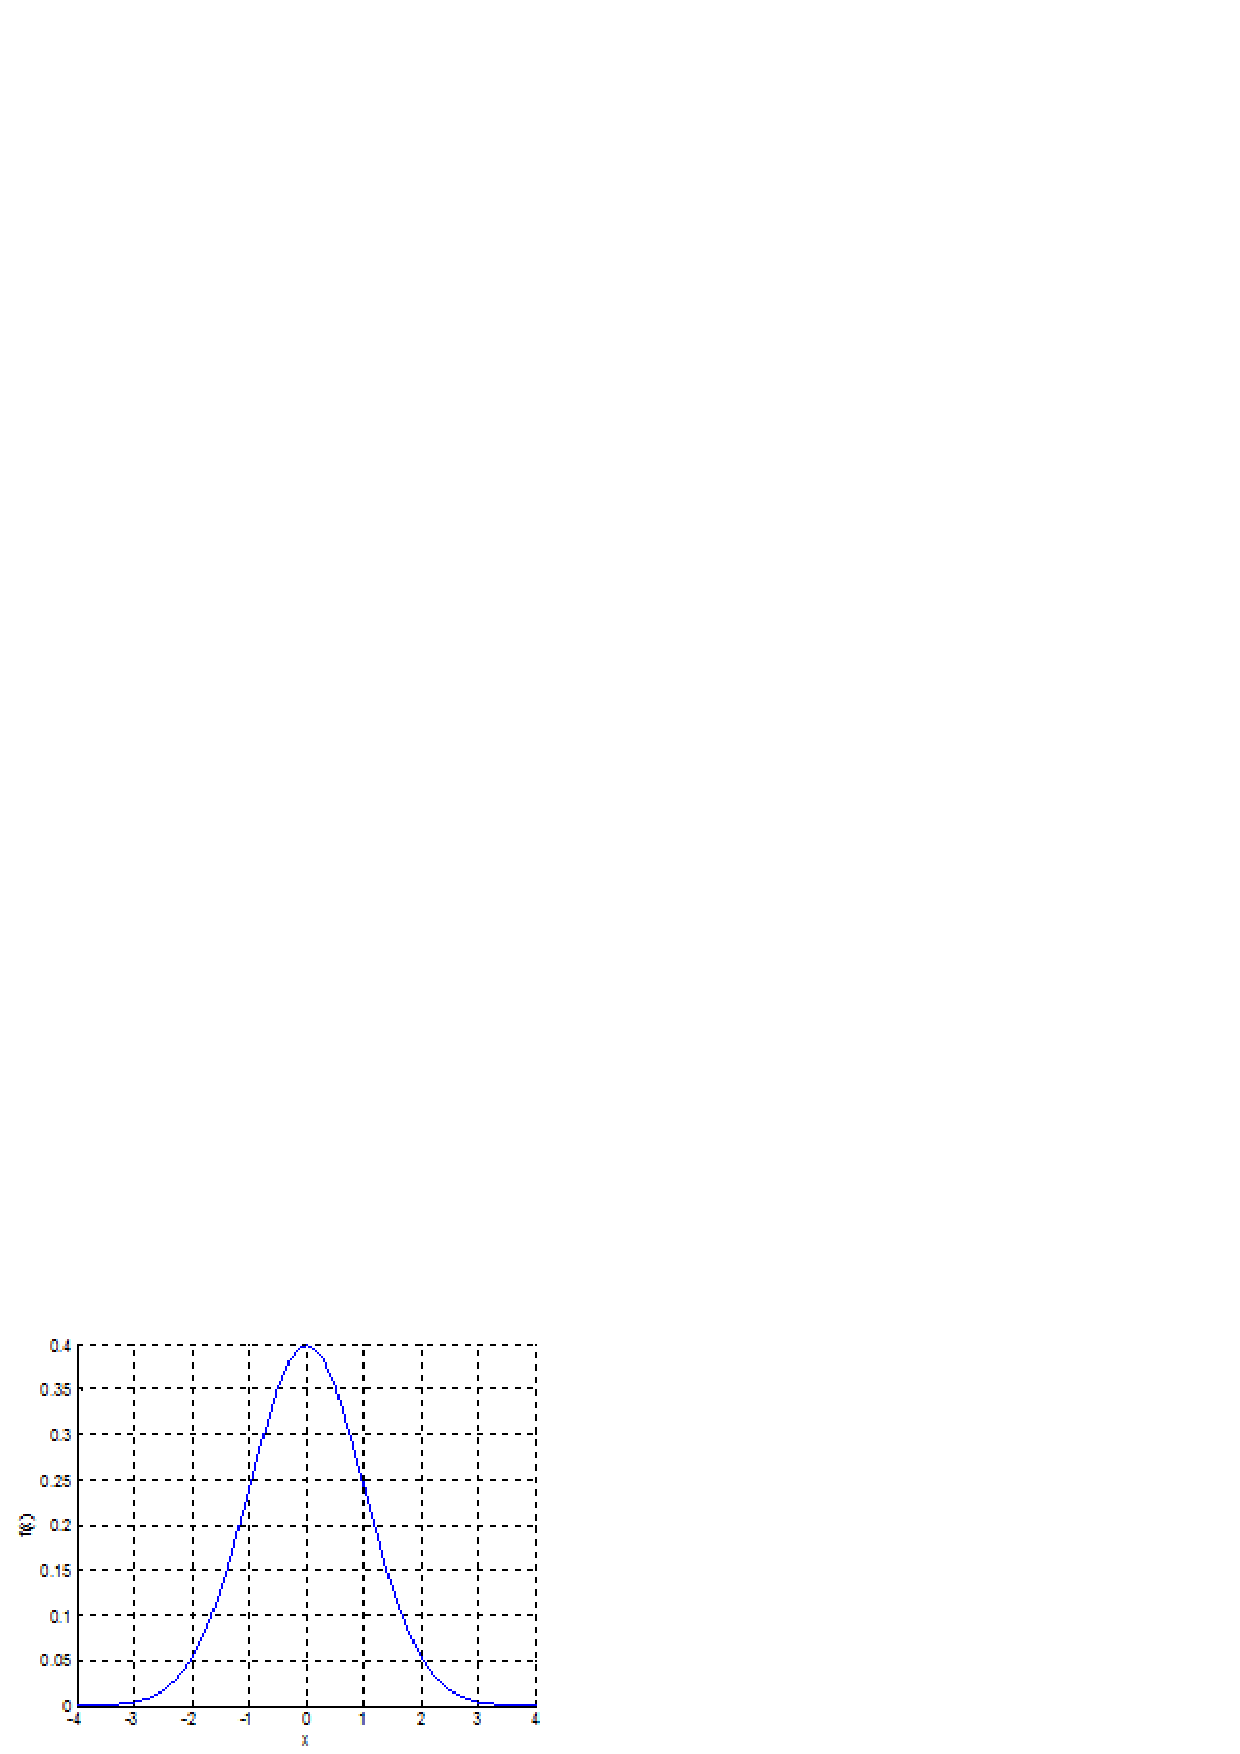
\includegraphics[width=0.55\columnwidth]{funcdesign_chapters/figloadmodels/image51.png}
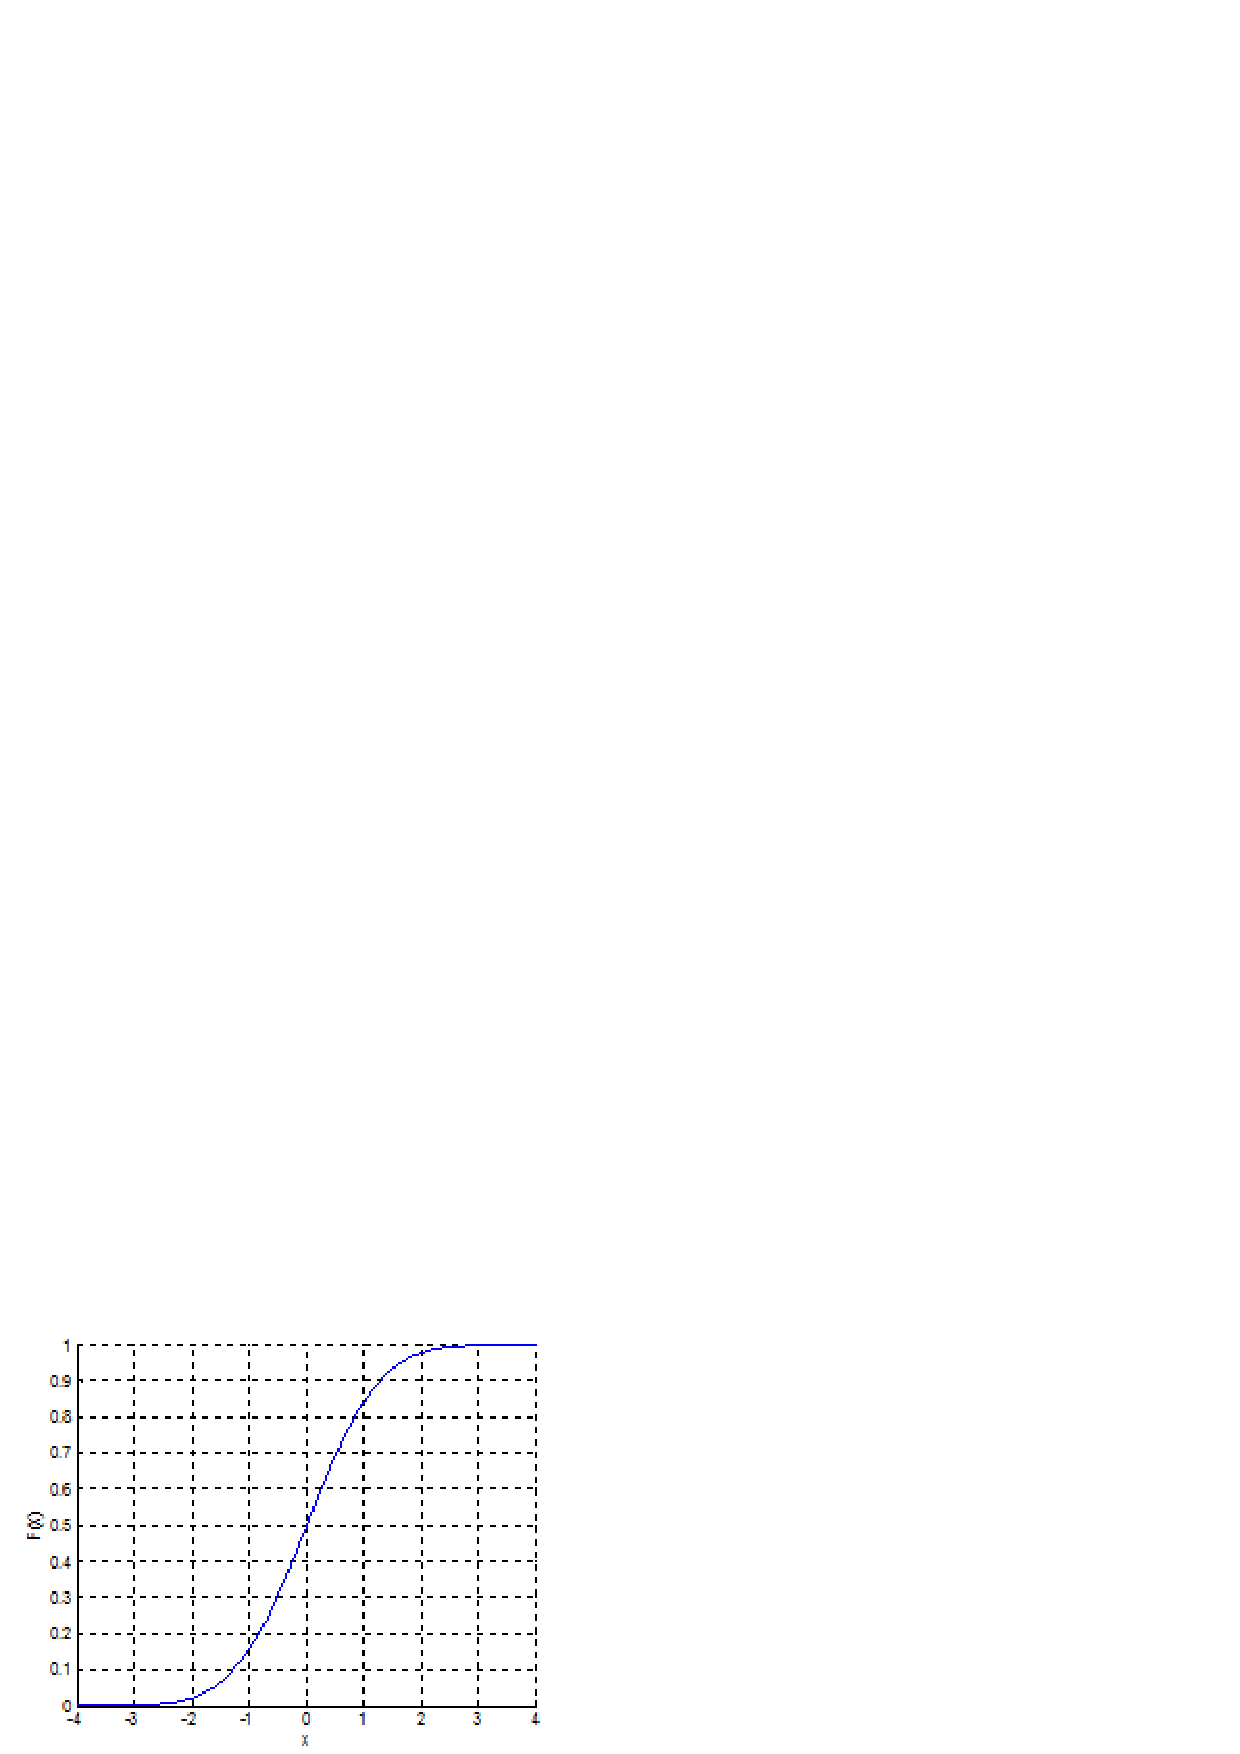
\includegraphics[width=0.55\columnwidth]{funcdesign_chapters/figloadmodels/image52.png}
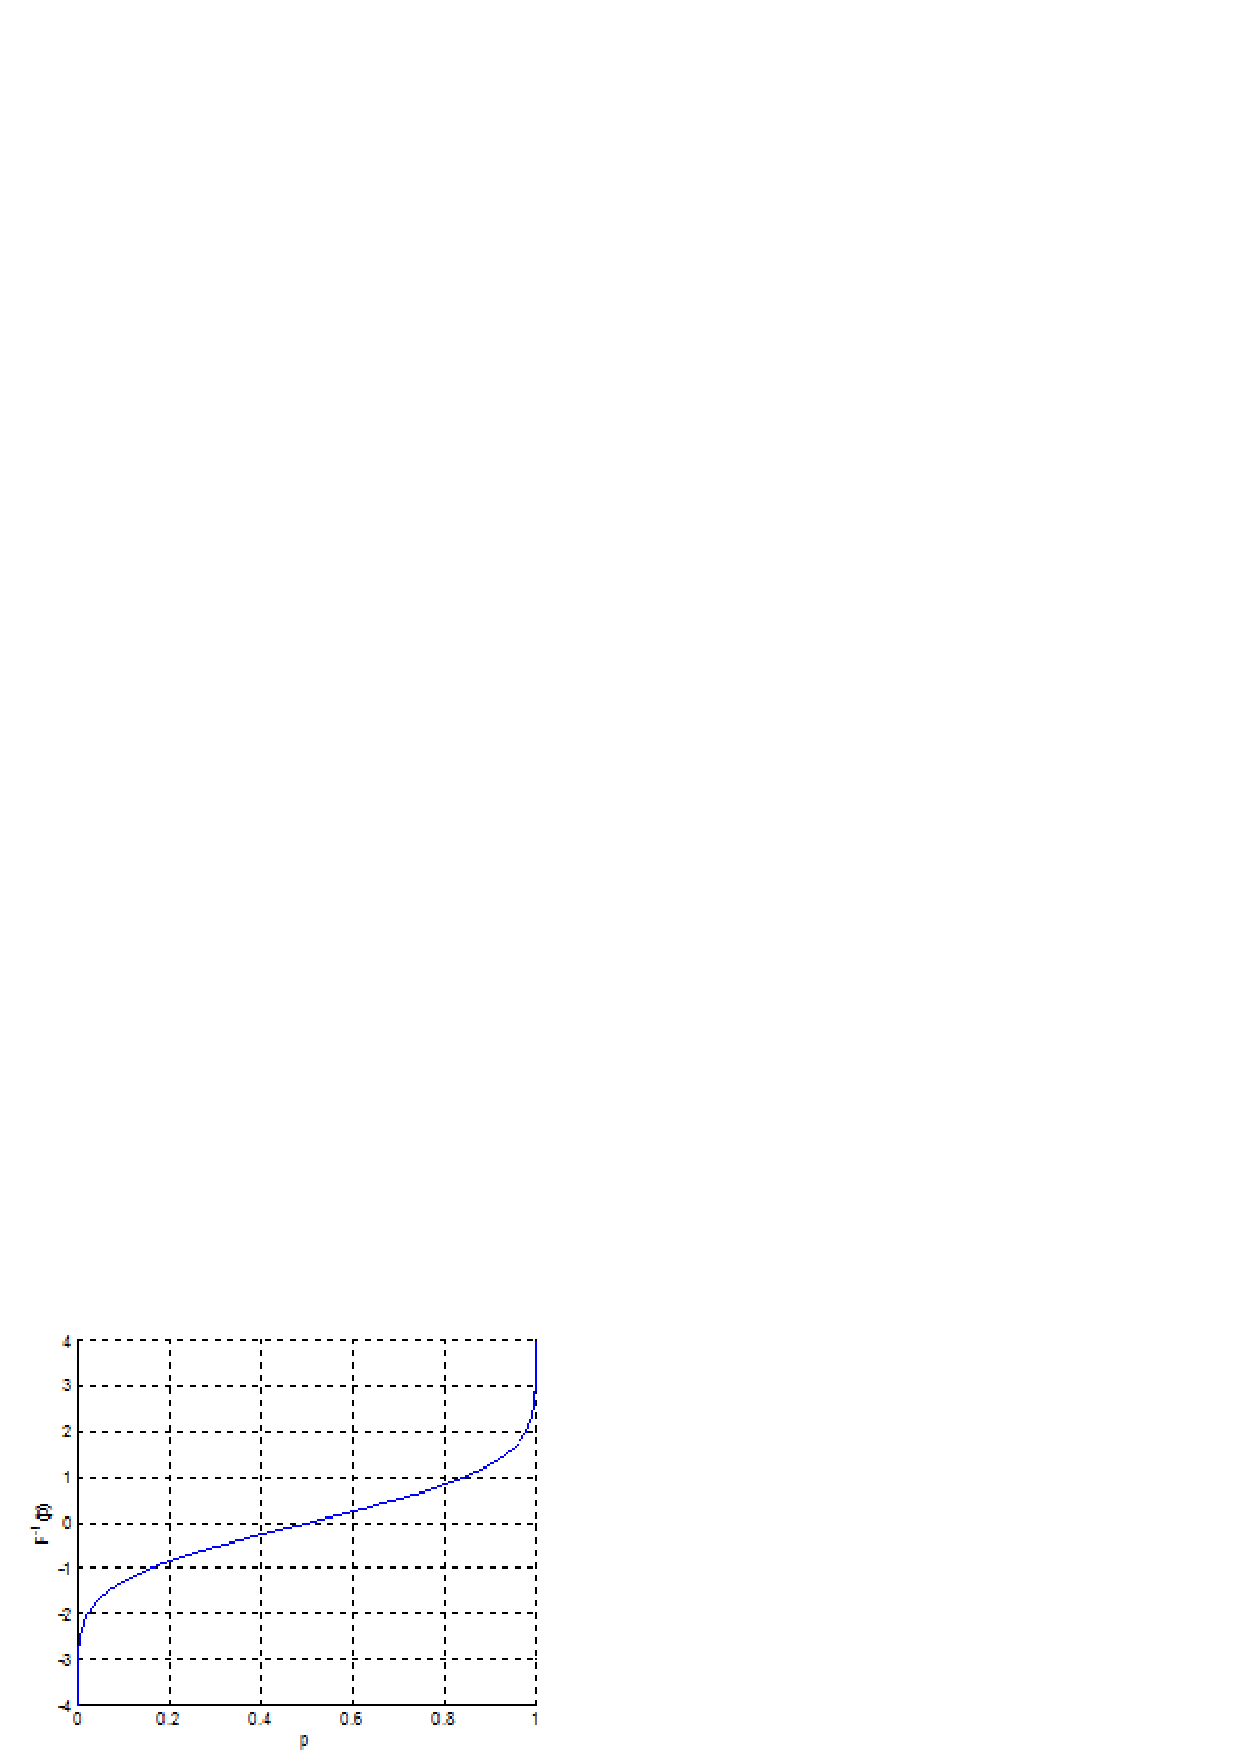
\includegraphics[width=0.55\columnwidth]{funcdesign_chapters/figloadmodels/image53.png}
\caption{PDF (top), CDF (middle) and inverse CDF (bottom) of the standard normal distribution function.}\label{fig:Figure_3.2}
\end{figure}

The CDF, $F(x)$, has the flowing properties:
\begin{enumerate}
\item $F(x)$ is non-decreasing;
\item $\lim_{x\rightarrow -\infty}F(x)=0$;
\item $\lim_{x\rightarrow \infty}F(x)=1$.
\end{enumerate}

Property 1 can be easily proven: if $x_1<x_2$, then $P[X\leq x_1] \leq P[X\leq x_2]$ and thus $F(x_1) \leq F(x_2)$. For a formal proof of properties 2 and 3, the reader is referred to \cite{GrimmettStirzaker1983}. But even without a proof it is intuitively clear that a realization from a probability function will be lower than $\infty$ and higher than -$\infty$.

Since $F(x)$ is non-decreasing, the inverse CDF, $F^{-1}(p)$, is also a non-decreasing function. In probabilistic computations, mainly the inverse CDF, $F^{-1}(x)$, of a variable $X$ is applied, as schematically depicted in \Fref{fig:Figure_3.3}. The library of distribution functions therefore mostly consists of inverse CDF's. The procedure of \Fref{fig:Figure_3.3} is explained below.

\begin{figure}[H]\centering
\includegraphics*[width=3.95in, height=2.59in, keepaspectratio=false]{funcdesign_chapters/figloadmodels/image54.png}
\caption{Procedure for determining a load variable associated with a randomly selected standard normally distributed variable ($u$-value), for the case of uncorrelated variables.}\label{fig:Figure_3.3}
\end{figure}

As described in section \Aref{Section_2.3}, random variables are represented by standardised $U$-variables in the probabilistic computations in the \probLib, and the function $Z(U)$ is explored to derive an estimate of the failure probability. In order to evaluate function $Z(U)$, the realisations of the $U$-variables are first translated to the corresponding realisations of the $X$-variables and subsequently the $Z$-value is determined. Assume for the sake of simplicity that the $X$-variables are mutually independent (correlations will be dealt with in \Aref{Section_3.4}). As explained in \Aref{Section_2.2.3}, the transformation from a realization, $u$, of variable $U$, to realization $x$, of variable $X$, is done in such a away that the (non-)exceedance probabilities of $u$ and $x$ are equal. This transformation, as depicted in \Fref{fig:Figure_3.3}, can be formulated as follows:
\begin{equation}
\Phi \left(u\right)=F\left(x\right)\; \quad \Rightarrow \; \quad x=F^{-1} \left(\Phi \left(u\right)\right) \label{ZEqnNum694082}
\end{equation}
where:

\begin{tabular}{lll}
$\Phi$ &=& standard normal distribution function\\
$F$ &=& CDF of variable $X$\\
$F^{-1}$ &=& inverse CDF of $X$\\
$x$ &=& realisation of $X$\\
$u$ &=& realisation of $U$\\
\end{tabular}

This procedure automatically guarantees that variable $x$ is a realization from distribution function $F(x)$ and therefore correctly represents the statistical properties of variable $X$. This is demonstrated below.

First it needs to be shown that the value $p = \Phi(u)$ is a realization from a standard uniform distribution function. The standard uniform distribution function is the CDF in which each value in the range $[0,1]$ has equal probability density. The CDF of this function is as follows (see also \Fref{fig:Figure_3.4}):
\begin{equation}
F\left(x\right)\; =\left\{\begin{array}{l} {0\quad ;x\le 0\quad } \\ {\; x\quad ;0<x<1} \\ {1\quad ;x\ge 1\quad } \end{array}\right. \quad \label{ZEqnNum892201}
\end{equation}

Consider a realization, $u^*$, of the standard normal distribution function with a probability of non-exceedance equal to $p^* = \Phi(u^*)$. By definition this means that the probability that a random sample $u$ from the standard normal distribution function does not exceed $u^*$ is equal to $p^*$. In formula:
\begin{equation}
P\left[u\le u^*\right]=p^* \label{ZEqnNum312921}
\end{equation}

Since $\Phi$ is a CDF, it is a non-decreasing function. Therefore it follows from equation \eqref{ZEqnNum312921} that:
\begin{equation}
P\left[\Phi \left(u\right)\le \Phi \left(u^*\right)\right]=p^*\label{3.6)}
\end{equation}

And since by definition $p^*= \Phi(u^*)$, this simplifies to:
\begin{equation}
P\left[\Phi \left(u\right)\le p^*\right]=p^* \label{3.7)}
\end{equation}

So the probability that $\Phi(u)$ does not exceed a given value $p^*$ ($0\leq p^* \leq 1$) is equal to $p^*$. This shows that $\Phi(u)$ is a realization from a standard uniform distribution function, as described by equation \eqref{ZEqnNum892201} and depicted in \Fref{fig:Figure_3.4}.

\begin{figure}[H]\centering
\includegraphics*[width=4.28in, height=3.21in, keepaspectratio=false]{funcdesign_chapters/figloadmodels/image55.png}
\caption{Standard uniform distribution function (CDF).}\label{fig:Figure_3.4}
\end{figure}

It has been demonstrated that the value $p$ in \Fref{fig:Figure_3.3} is a realization from the standard uniform distribution function. The next step is to show that the value $x = F^{-1}(p)$ in \Fref{fig:Figure_3.3} is a realization from distribution function $F(x)$. For this purpose, consider a value $x^*$ with probability of non-exceedance $p^*$. This means: $F(x^*) = p^*$ and $x^* = F^{-1}(p^*)$. The value $p$ in \Fref{fig:Figure_3.3} is taken from a standard uniform distribution function (as proven above), which means:
\begin{equation}
P\left[p\le p^*\right]=p^*\label{ZEqnNum788001}
\end{equation}

Since $F$ is an inverse CDF, it is a non-decreasing function and therefore it follows from equation \eqref{ZEqnNum788001} that:
\begin{equation}
P\left[F^{-1} \left(p\right)\le F^{-1} \left(p^*\right)\right]=p^*\label{ZEqnNum178723} 
\end{equation}

By definition $x^* = F^{-1}(p^*)$ and $x = F^{-1}(p)$, which means equation \eqref{ZEqnNum178723} simplifies to:
\begin{equation}
P\left[x\le x^*\right]=p^*\label{3.10)} 
\end{equation}

Since $p^*= F(x)$, this means: 
\begin{equation} 
P\left[x\le x^*\right]=F\left(x^*\right)\label{3.11)} 
\end{equation}

This shows that value $x$ in \Fref{fig:Figure_3.3} is a realization from distribution function $F(x)$. 

\Note{the \probLib works with standard normalized $U$-variables. The limit state function $Z(U)$ is explored to derive an estimate of the failure probability. In order to evaluate function $Z(U)$, the realisations of the $U$-variables are first translated to the corresponding realisations of the $X$-variables to be able to determine the $Z$-value. In this transformation, the inverse CDF of variable $X$ is applied, to provide variable $X$ with the correct statistical properties.}

\Note{\Aref{app:distributionfunctions} presents distribution functions available in the \probLib.The library contains the ''inverse cumulative distribution functions'' which means the input consists of a probability, $p$, of non-exceedance and the output consist of the associated realization, $x$, of the variable that is described with this distribution function.} 

%Besides $p$, the input of the inverse CDF's also consists of a set of parameter values $\theta = (\theta_1, \dots ,\theta_n)$. These parameter values quantify the relation between $p$ and $x$. Note that the value of $n$ can be different for different distribution functions, as shown in the second column of \Tref{Table_3.1}. Each distribution function as mentioned in \Tref{Table_3.1} has a fixed number, $n$, of parameters but the values of these parameters will be different for different variables. So, for instance, it is possible to describe both river discharge and sea water level with the lognormal distribution, but the values of the two parameters of this distribution function for river discharge will be different from the values that are used for sea water level. In other words: the same module can be used to describe probabilities of different random variables and differences between the variables are characterized by differences in parameter values. 

\section{Probability distribution functions}\label{app:distributionfunctions}

\subsection{Deterministic distribution\label{sec:deterministicdistribution}}

A deterministic random variable takes a certain value, let's say value $x_0$, with probability $1$. The cumulative distribution function of such variable is given as follows:
\begin{align}
F(x) = \left\{\begin{array}{l} {1\mbox{ for }x\geq x_0} \\ {0 \mbox{ for }x<x_0} \end{array}\right.
\end{align}

\subsection{Uniform distribution\label{sec:uniformdistribution}}

The probability density function for the uniform distribution is given by:
\begin{align}
f\left(x\right)=\left\{\begin{array}{l} {\frac{1}{b-a}\mbox{ for }a\le x\le b} \\ {0\mbox{ for }x<a\mbox{ or }x>b} \end{array}\right. \label{4.72)} 
\end{align}

The corresponding cumulative distribution function is given by: 
\begin{align}
F\left(x\right)=\left\{\begin{array}{l} {0\mbox{ for }x<a} \\ {\frac{x-a}{b-a} \mbox{ for }a\le x<b} \\ {1\mbox{ for }x\ge b} \end{array}\right. \label{4.73)} 
\end{align}

The inverse of the uniform distribution is given by:
\begin{align}
F^{-1} \left(p\right)=a+p\left(b-a\right),    p\in \left(0,1\right) \label{4.74)} 
\end{align}

The inverse, $F^{-1}$, gives the value of $x$ associated for a given value of the probability of non-exceedance, $p$. 

The distribution parameters a and $B$ indicate the range over which the probability density function is non-zero, with a indicating the starting point and $B$ indicating the ending point. \Fref{fig:A.1} and \Fref{fig:A.2} show the uniform probability density and cumulative probability distribution, respectively, as a function of a and b. 

\begin{figure}[H]\centering
\includegraphics*[width=3.04in, height=2.33in, keepaspectratio=false]{funcdesign_chapters/figappdistributionfunctions/image30}
\caption{Uniform probability density function, with parameters $a$ and $B$ indicated}\label{fig:A.1}
\end{figure}

\begin{figure}[H]\centering
\includegraphics*[width=2.85in, height=2.34in, keepaspectratio=false]{funcdesign_chapters/figappdistributionfunctions/image31}
\caption{Uniform cumulative distribution function, with parameters $a$ and $B$ indicated}\label{fig:A.2}
\end{figure}


\subsection{Normal distribution\label{sec:normaldistribution}}
The probability density function for the normal distribution is given by:
\begin{align}
f\left(x\right)=\frac{1}{\sqrt{2\pi \sigma ^{2} } } \exp \left[-\frac{\left(x-\mu \right)^{2} }{2\sigma ^{2} } \right] \label{4.75)} 
\end{align}

The corresponding cumulative distribution function is given by: 
\begin{align}
F\left(x\right)=\frac{1}{2} \left[1+\mbox{erf}\left(\frac{x-u}{\sqrt{2\sigma ^{2} } } \right)\right] \label{4.76)} 
\end{align}

where erf refers to the error function, which is expressed as follows:
\begin{align}
\mbox{erf}\left(x\right)=\frac{2}{\sqrt{\pi } } \int _{0}^{x}e^{-t^{2} } dt \label{4.77)} 
\end{align}

The standard normal distribution, denoted by $\Phi$, is the special case of the normal distribution for which the mean is equal to zero and the standard deviation is equal to one. For the special case of the standard normal distribution, the inverse is given as follows: 
\begin{align}
\Phi ^{-1} \left(p\right)=\sqrt{2} \cdot \textrm{erf}^{-1} \left(2p-1\right),   p\in \left(0,1\right) \label{ZEqnNum712080} 
\end{align}

For the general case of a normal distribution with mean $\mu $ and standard deviation $\sigma $, the inverse is given as follows:
\begin{align}
F^{-1} \left(p;\mu ,\sigma ^{2} \right)=\mu +\sigma \cdot \Phi ^{-1} \left(p\right),   p\in \left(0,1\right) \label{ZEqnNum182159} 
\end{align}

\Note{there is no explicit form for the normal distribution or inverse normal distribution;
therefore, these functions need to be approximated numerically. The method implemented in the \probLib is described in \Aref{appConversions}.}

\Fref{fig:A.3} shows the probability density of the normal distribution, with the parameters $\mu $ and $\sigma $ indicated. \Fref{fig:A.4} shows the variation in the density function for different choices of $\mu $ and $\sigma $.

\begin{figure}[H]\centering
\includegraphics*[width=2.76in, height=2.33in, keepaspectratio=false]{funcdesign_chapters/figappdistributionfunctions/image32}
\caption{Normal probability density function, with parameters $\mu $ and $\sigma $ indicated}\label{fig:A.3}
\end{figure}

\begin{figure}[H]\centering
\includegraphics*[width=4.10in, height=3.22in, keepaspectratio=false]{funcdesign_chapters/figappdistributionfunctions/image33}
\caption{Illustration of the effect of parameters $\mu $ and $\sigma $}\label{fig:A.4}
\end{figure}


\subsection{(Shifted) Lognormal distribution\label{sec:lognormaldistribution}}
The lognormal distribution is a probability distribution of a random variable whose logarithm is normally distributed. That is, if $x$ is a random variable with a lognormal distribution, then $Y$ = log($x$) is normally distributed, and similarly if $Y$ is a random variable with a normal distribution, exp(y) is lognormally distributed.

The lognormal density function is given as follows:
\begin{align}
f\left(x;\mu ,\sigma ,\varepsilon \right)=\frac{1}{\left(x-\varepsilon \right)\sqrt{2\pi \sigma ^{2} } } \exp \left[-\frac{\left(\ln \left(x-\varepsilon \right)-\mu \right)^{2} }{2\sigma ^{2} } \right],    x>0 \label{4.80)} 
\end{align}
%\todo{ddierman3:what is the added value of $\varepsilon$? It seems $\mu$ suffices for the shift}

The corresponding cumulative distribution function is given by: 
\begin{align}
F\left(x\right)=\Phi \left(\frac{\ln \left(x-\varepsilon \right)-\mu }{\sigma } \right) \label{4.81)} 
\end{align}

where $\Phi$ is the standard normal distribution function described in \Aref{sec:normaldistribution}. 

The parameters of the lognormal distribution, $\mu $ and $\sigma $, are the mean and standard deviation of the associated normally distributed variable. That is, if $x$ is lognormally distributed, and $Y$ = log($x$) is normally distributed, the lognormal parameters $\mu $ and $\sigma $ are the mean and standard deviation of y. The parameter $\varepsilon $ is the shift parameter and serves to horizontally translate the distribution. \Fref{fig:A.5} shows the effect of different choices of the parameters.

\begin{figure}[H]\centering
\includegraphics*[width=4.10in, height=3.22in, keepaspectratio=false]{funcdesign_chapters/figappdistributionfunctions/image34}
\caption{Illustration of the effect of parameters $\mu $, $\sigma $, and $\varepsilon $ on the lognormal density function}\label{fig:A.5}
\end{figure}

To get the inverse distribution, the following steps are taken. The first step is, for a given probability p, the inverse standard normal variable is computed by numerically solving equation \eqref{ZEqnNum712080}. The associated normal variable with mean $\mu $ and standard deviation $\sigma $ is then computed analytically using equation \eqref{ZEqnNum182159}. The relationship between the normal and lognormal distributions is then exploited:
\begin{align}
F^{-1} \left(p;\mu ,\sigma \right)=\exp \left[\mu +\sigma \cdot \Phi ^{-1} \left(p\right)\right]+\varepsilon ,    p\in \left(0,1\right)\label{4.82)} 
\end{align}

\subsection{(Shifted) Exponential distribution\label{sec:exponentialdistribution}}
The density function for the shifted exponential distribution is given as follows:
\begin{align}
f\left(x;\lambda ,\varepsilon \right)=\left\{\begin{array}{l} {\lambda \exp \left[-\lambda \cdot \left(x-\varepsilon \right)\right],    x>\varepsilon } \\ {0,                                          x<\varepsilon } \end{array}\right. \label{4.83)} 
\end{align}

The corresponding cumulative distribution function is given by: 
\begin{align}
F\left(x;\lambda ,\varepsilon \right)=\left\{\begin{array}{l} {1-\exp \left[-\lambda \cdot \left(x-\varepsilon \right)\right],    x\ge \varepsilon } \\ {0\qquad\qquad\qquad\qquad\qquad ,x<\varepsilon } \end{array}\right. \label{4.84)} 
\end{align}

The inverse distribution can be analytically computed from the distribution function:

 
\begin{align}
F^{-1} \left(p;\lambda ,\varepsilon \right)=\varepsilon -\frac{\ln \left(1-p\right)}{\lambda } . \label{4.85)} 
\end{align}

The parameter of the exponential distribution, $\lambda $, is referred to as a rate parameter, and determines how quickly the density function goes to zero. The parameter $\varepsilon $ is the shift parameter and serves to horizontally translate the density. \Fref{fig:A.5} shows the effect of different choices of the parameters.

\begin{figure}[H]\centering
\includegraphics*[width=4.17in, height=3.27in, keepaspectratio=false]{funcdesign_chapters/figappdistributionfunctions/image35}
\caption{Illustration of the effect of parameters $\lambda $ and $\varepsilon $ on the exponential density function}\label{fig:A.6}
\end{figure}



\subsection{Gumbel distribution\label{sec:gumbeldistribution}}
The Gumbel distribution is one of three cases of the generalized extreme value distribution. It is often used to model the distribution of block maxima. 

The probability density function is expressed as follows:
\begin{align}
f\left(x;\alpha ,\xi \right)=\frac{1}{\alpha } \exp \left[-\frac{1}{\alpha } \left(x-\xi \right)\right]\cdot \exp \left[-\exp \left[-\frac{1}{\alpha } \left(x-\xi \right)\right]\right] \label{4.86)} 
\end{align}

The corresponding cumulative distribution function is given by: 
\begin{align}
F\left(x;\alpha ,\xi \right)=\exp \left[-\exp \left[-\frac{1}{\alpha } \left(x-\xi \right)\right]\right]\label{ZEqnNum826654} 
\end{align}

The inverse distribution can be analytically computed from the distribution function:

 
\begin{align}
F^{-1} \left(p;\alpha ,\xi \right)=\xi -\alpha \ln \left(\ln \left(p\right)\right)\label{4.88)} 
\end{align}

The parameters of the gumbel distribution, $\alpha $ and $\xi $, are referred to as the scale and location parameters, respectively. These two parameters can be written in terms of the mean (E($x$)) and standard deviation ($\sigma $($x$)), or in the case of a sample selection, of the sample. The mean and standard deviation of the gumbel distribution are given as follows:
\begin{align}
E\left(x\right)&=\xi +\gamma \alpha \label{ZEqnNum262731} \\ 
\sigma \left(x\right)&=\frac{\alpha \pi }{\sqrt{6} } \label{ZEqnNum724056} 
\end{align}

Equations \eqref{ZEqnNum262731} and \eqref{ZEqnNum724056} can be used to solve for the parameters $\alpha $ and $\xi $. First, $\alpha $ is solved in terms of the standard deviation (equation \eqref{ZEqnNum864535}), and subsequently, equations \eqref{ZEqnNum262731} and \eqref{ZEqnNum864535} are used in combination to solve $\xi $ in terms of the mean and standard deviation. 
\begin{align}
\alpha &=\frac{\sigma \left(x\right)\cdot \sqrt{6} }{\pi } \label{ZEqnNum864535} \\  
\xi &=E\left(x\right)-\gamma \cdot \frac{\sigma \left(x\right)\cdot \sqrt{6} }{\pi } \label{4.92)} 
\end{align}

The \probLib supports two types of input: either the set of parameters, or the mean and standard deviation. An important note is that the \probLib works with the rate parameter instead of the scale parameter. The rate parameter is equal to the reciprocal of the scale parameter; that is: 
\begin{align}
\textrm{rate parameter}=\frac{1}{\textrm{scale parameter}} \label{4.93)} 
\end{align}

The two parameters that should be input into the \probLib are therefore the rate parameter and the location parameter. \Fref{fig:A.7} shows the effect of different choices of the parameters.

\begin{figure}[H]\centering
\includegraphics*[width=4.17in, height=3.27in, keepaspectratio=false]{funcdesign_chapters/figappdistributionfunctions/image36}
\caption{Effect of the scale and location parameters, $\alpha $ and $\xi $, on the Gumbel density function}\label{fig:A.7}
\end{figure}


\subsection{Gamma distribution\label{sec:gammadistribution}}
A random variable $X$ that is gamma-distributed with shape $k$ and scale $\theta$ is denoted by $X \sim \Gamma (k,\theta)$. The probability density function is parameterized as:
\begin{equation}
f(x;k,\theta) = \frac{x^{k-1} e^{-x/\theta}}{\theta^k \Gamma(k)} \hspace{1cm} \textrm{for} \hspace{1cm} x>0 \hspace{1cm} \textrm{and} \hspace{1cm} (k, \theta )>0
\end{equation}
with $\Gamma(k)$ the \emph{gamma function} (not to be confused with the Gamma distribution itself). The cumulative distribution function is the regularized gamma function:
\begin{equation}
F(x;k,\theta) = \int_0^x f(u;k,\theta) \textrm{d} u = \frac{\gamma (k, x/\theta)}{\Gamma(k)}
\end{equation}
in which $\gamma (k, x/\theta)$ is the lower incomplete gamma function. The cumulative distribution function is expressible as a infinite series, utilizing $k$ as a positive integer:
\begin{equation}
F(x;k,\theta) = e^{-x/\theta} \sum_{i=k}^{\infty} \frac{1}{i!} \left( \frac{x}{\theta} \right)^i
\end{equation}
Alternatively, the Gamma distribution can be written using the shape parameter $\alpha = k$ and the rate $\beta = 1 / \theta$. In that case, we have:
\begin{equation}
F(x;\alpha,\beta) = e^{-\beta x} \sum_{i=\alpha}^{\infty} \frac{(\beta x)^i}{i!}
\end{equation}


\subsection{Weibull distribution\label{sec:weibulldistribution}}
The probability density function of a Weibull random variable $x \geq 0$ holds:
\begin{equation}
f(x;\lambda,k) = \frac{k}{\lambda} \left( \frac{k}{\lambda} \right)^{k-1} e^{-(x / \lambda)^k}
\end{equation}
and $f(x;\lambda,k) = 0$ for $x < 0$. In this expression, $k>0$ is the shape parameter and $\lambda > 0$ the scale parameter of the distribution. The cumulative distribution function of a Weibull random variable $x \geq 0$ yields:
\begin{equation}
F(x;\lambda,k) = 1 - e^{-(x / \lambda)^k}
\end{equation}
and $F(x;\lambda,k) = 0$ for $x < 0$. A value $k < 1$ indicates that the failure rate decreases over time; likewise, a value $k>1$ indicates that the failure rate increases with time.


\subsection{Rayleigh distribution\label{sec:rayleighdistribution}}
The probability density function of the Rayleigh distribution of a random variable $x \geq 0$ holds:
\begin{equation}
f(x;\sigma) = \frac{x}{\sigma^2} e^{-x^2/(2 \sigma^2)}
\end{equation}
in which $\sigma$ represents the scale parameter of the distribution. The cumulative distribution function for this random variable $x \geq 0$ holds:
\begin{equation}
F(x;\sigma) = 1-e^{-x^2/(2 \sigma^2)}
\end{equation}
Notice that the Weibull distribution is a generalization of the Rayleigh distribution; in this instance, the parameter $\sigma$ is related to the Weibull scale parameter $\lambda$ through $\lambda = \sigma \sqrt{2}$. Notice, moreover, that a random variable $R$ is Rayleigh distributed if $R = \sqrt{X^2 + Y^2}$ and $X \sim N(0, \sigma^2)$ and $Y \sim N(0, \sigma^2)$, in which $N$ represents the normal distribution.


\subsection{Rayleigh-$N$ distribution\label{sec:rayleighNdistribution}}
The Rayleigh-$N$ distribution is a special distribution implemented in the \probLib. This distribution is based on the Rayleigh distribution (see \Aref{sec:rayleighdistribution}) and it is defined as follows:
\begin{equation}
F(x;\sigma,N) = \left(1-e^{-x^2/(2 \sigma^2)}\right)^N\mbox{ for $x\geq 0$}
\end{equation}
where $\sigma>0$ is the scale parameter and $N>0$. The Rayleigh-$N$ distribution is in fact the Rayleigh distribution taken to the power $N$. When $N=1$, the Rayleigh-$N$ distribution is exactly equal to the Rayleigh distribution. The corresponding probability density function is:
\begin{equation}
f(x;\sigma,N) = \frac{N x}{\sigma^2}\left(1-e^{-x^2/(2 \sigma^2)}\right)^{N-1} e^{-x^2/(2 \sigma^2)}\mbox{ for $x\geq 0$}
\end{equation}


\subsection{Pareto distribution\label{sec:paretodistribution}}
The probability density function of a Pareto random variable $x \geq x_m$ holds:
\begin{equation}
f(x;\alpha) = \frac{\alpha x_m^{\alpha}}{x^{\alpha + 1}}
\end{equation}
and $f(x;\alpha) = 0$ for $x < x_m$. In this expression, $\alpha > 0$ is a positive parameter and $x_m > 0$. The cumulative distribution function of a Pareto random variable $x \geq x_m$ yields:
\begin{equation}
F(x;\alpha) =  1 - \left( \frac{x_m}{x}  \right)^{\alpha}
\end{equation}
and $F(x;\alpha) = 0$ for $x < x_m$. 


\subsection{Triangular distribution\label{sec:triangulardistribution}}
The triangular distribution is indicated this way for the triangular shape of the probability density function. The probability density function of the random variable $x$ has a minimum (equal to 0) at $x = a$ and $x = b$, and has a maximum at $x = c$ equal to the value $2/(b-a)$.




\subsection{Conditional Weibull distribution\label{sec:conditionalweibulldistribution}} 

The conditional Weibull distribution gives the probability that $X=x$ conditionally on the event that $X>\omega $, where $\omega $ represents a threshold. It is used in when considering a peaks-over-threshold (POT) method. The distribution function of the conditional Weibull is given as follows:
\begin{align}
P\left(X\le x|X>\omega \right)=1-\exp \left[\left({\omega \mathord{\left/ {\vphantom {\omega  \sigma }} \right. \kern-\nulldelimiterspace} \sigma } \right)^{\xi } -\left({x\mathord{\left/ {\vphantom {x \sigma }} \right. \kern-\nulldelimiterspace} \sigma } \right)^{\xi } \right]\label{ZEqnNum182046} 
\end{align}

where the parameters $\omega $, $\sigma $, and $\xi $ refer to the threshold, scale, and shape parameter, respectively. The conditional Weibull distribution is often described in terms of exceedance frequencies rather than probabilities. The exceedance frequency of $x$ can be described as follows:
\begin{align}
Fr\left(X>x\right)=\lambda \cdot P\left(X>x|X>\omega \right)\label{ZEqnNum277845} 
\end{align}

where Fr refers to `frequency', and $\lambda $ is the frequency with which the selected threshold $\omega $ is exceeded:
\begin{align}
\lambda =Fr\left(X>\omega \right)\label{4.98)} 
\end{align}

In practice, $\lambda $ is determined by counting the number of independent peaks above the threshold and dividing by the number of years of record.

Expanding equation \eqref{ZEqnNum277845} so that the probability is full written out gives the following form of the exceedance frequency distribution for the condition Weibull:
\begin{align}
Fr\left(X>x\right)=\lambda \exp \left[\left({\omega \mathord{\left/ {\vphantom {\omega  \sigma }} \right. \kern-\nulldelimiterspace} \sigma } \right)^{\xi } -\left({x\mathord{\left/ {\vphantom {x \sigma }} \right. \kern-\nulldelimiterspace} \sigma } \right)^{\xi } \right]\label{4.99)} 
\end{align}

\subsection{Modified Gumbel\label{sec:modifiedgumbeldistribution}}

The form of the modified Gumbel is identical to the Gumbel distribution (see equation \eqref{ZEqnNum826654}), only the argument:
\[\frac{1}{\alpha } \left(x-\xi \right)\] 
is replaced by a 2$^{nd}$-degree polynomial. The function for the modified Gumbel is given by: 
\begin{align}
F\left(x;K_{r} \right)=\exp \left[-\exp \left[-K_{r} (x;a,b,c)\right]\right]\label{ZEqnNum838972} 
\end{align}

The polynomial $K_r$ is given as:
\begin{align}
K_{r} \left(x;a,b,c\right)=ax^{2} +bx+c\label{ZEqnNum393716} 
\end{align}

The parameters of the modified Gumbel are the coefficients of $K_r$: $a$, $b$, and $c$.  

The modified Gumbel is not a probability distribution; equation \eqref{ZEqnNum838972} does not necessarily span the range from $0$ to $1$, and the area under the density does not sum to $1$. Rather it is a function that approximates the distribution of the wind speed. The parameters of the function (a, b, and c) were chosen to ensure this agreement. However, the agreement is only valid for particular ranges of the wind speed. \Fref{fig:A.9} and \Fref{fig:A.10} show the modified Gumbel for the wind station Deelen, shown over two diferent ranges of wind speeds. The former shows the functions over the range $0$ to $40$ m/s, and the probability density and distribution function appear to be reasonable approximations. The latter shows that for negative wind speeds, rather than the density and the non-exceedance probability being zero, they display peculiar behavior. This illustrates that these functions are not distributions/density functions, and should therefore be used with care, such that only wind speeds in the valid range are considered.

\begin{figure}[H]\centering
\includegraphics*[width=3.07in, height=2.40in, keepaspectratio=false]{funcdesign_chapters/figappdistributionfunctions/image38}
\caption{ Modified Gumbel for wind station Deelen, shown over the range of wind speeds $0$ to 40 m/s}\label{fig:A.9}
\end{figure}

\begin{figure}[H]\centering
\includegraphics*[width=3.12in, height=2.40in, keepaspectratio=false]{funcdesign_chapters/figappdistributionfunctions/image39}
\caption{ Modified Gumbel for wind station Deelen, shown over the range of wind speeds -40 to 40 m/s}\label{fig:A.10}
\end{figure}

To solve for the inverse of the modified Gumbel, equation \eqref{ZEqnNum838972} is rearranged:
\begin{align}
K_{r} =\ln \left[-\ln \left(p\right)\right]\label{4.102)} 
\end{align}

where $p$ is the non-exceedance probability. Substituting equation \eqref{ZEqnNum393716} for $K_r$ gives the following:
\begin{align}
ax^{2} +bx+c=\ln \left[-\ln \left(p\right)\right]\to ax^{2} +bx+c'=0\label{ZEqnNum294065} 
\end{align}

where $c'$ is given as:
\begin{align}
c'=c+\ln \left[-\ln \left(p\right)\right]\label{4.104)} 
\end{align}

The inverse of the modified Gumbel can then be solved using the quadratic equation:
\begin{align}
F^{-1} \left(p;a,b,c\right)=\left\{\begin{array}{l} {\frac{-b+\sqrt{b^{2} -4ac'} }{2a} ,    \left(b^{2} -4ac'\right)>0} \\ {\frac{-b}{2a} ,                                    \left(b^{2} -4ac'\right)<0  } \end{array}\right. \label{ZEqnNum802912} 
\end{align}

Note that this solution is pragmatic in the sense that only one half of the quadratic solution is used, based on the knowledge that wind speeds are not negative (note that typically the quadratic solution is $(-b \pm \sqrt{b^2 - 4ac})/2a$, and here we ignore the minus). Also, in cases where the square root term is negative, there are no real solutions; what is done in this case is to take the value at the peak (or trough) of the parabola, as this point will be the closest to the $x = 0$ axis. To illustrate this, \Fref{fig:A.11} shows the quadratic equation given by formula \eqref{ZEqnNum294065} for six different values of the non-exceedance probability $p$. 

In \Fref{fig:A.10} it was shown that for non-exceedance probabilities less than about 0.35, there is no solution to the inverse. It is for these cases that the square-root term in formula \eqref{ZEqnNum802912} is negative, and the second term $-b/2a$ is used as an approximate solution. This is evident in the first two subplots of \Fref{fig:A.11}, where the parabola does not cross the $x = 0$ line. 

\begin{figure}[H]\centering
\includegraphics*[width=3.90in, height=3.04in, keepaspectratio=false]{funcdesign_chapters/figappdistributionfunctions/image40}
\caption{Quadratic equation \eqref{ZEqnNum294065} for wind station Deelen, shown for six different non-exceedance probabilities (indicated in figure). The red vertical line indicates the solution to the inverse by equation \eqref{ZEqnNum802912}}\label{fig:A.11}
\end{figure}


\subsection{Truncated Gumbel distribution\label{sec:truncatedgumbeldistribution}}
The truncated Gumbel distribution is used in the correlation model Volker, and is therefore described in this section. Recall the form of the Gumbel distribution function (equation \eqref{ZEqnNum826654}), shown below for the case of a location parameter equal to zero and a scale parameter equal to $1$: 
\begin{align}
F\left(x\right)=\exp \left[-\exp \left(-x\right)\right]\label{4.106)} 
\end{align}

A truncated Gumbel distribution has the following form: 
\begin{align}
F\left(x;d\right)=\left\{\begin{array}{l} {\frac{1}{1-d} \exp \left[-\exp \left(-x\right)\right],    x\le x_{d} } \\ {1\qquad\qquad\qquad\qquad, x>x_{d} } \end{array}\right. \label{ZEqnNum480192} 
\end{align}

Setting the non-exceedance probability to $1$ for values of $x$ greater than $x_d$ essentially truncates the probability that values higher than $x_d$ will be observed. That is, the probability density of $x$ values higher than $x_d$ will be equal to zero. The ratio 1/(1 -- $d$) normalizes the distribution and that ensures that the total probability is equal to $1$. The value of d can be though of as the fraction of the distribution that will be truncated. That is, if $d = 0.02$, the highest $2$\% of the distribution will be truncated.

The endpoint of the distribution, $x_d$, can be derived from equation \eqref{ZEqnNum480192} and is given as follows:
\begin{align}
x_{d} =-\ln \left[-\ln \left(1-d\right)\right]\label{4.108)} 
\end{align}

\begin{figure}[H]\centering
\includegraphics*[width=3.11in, height=2.48in, keepaspectratio=false]{funcdesign_chapters/figappdistributionfunctions/image41}
\caption{ Illustration of the effect of including the truncation factor $d>0$ in equation \eqref{ZEqnNum480192}, here shown for $d = 0.02$}\label{fig:A.12}
\end{figure}

\subsection{Truncated normal distribution\label{sec:truncatednormaldistribution}}

The truncated normal distribution is a normal distribution between
a lower and upper boundary and zero elsewhere.
It is defined by the parameters $\mu, \sigma, a, b$,
respectively the mean, deviation, lower boundary and upper boundary,
all relative to the underlying normal distribution.

The distribution function is equal to the normal distribution function between the boundaries,
but corrected with a factor $\alpha$ to obtain a normalized function.

This correction factor can be calculated easily by using the cumulative value below
the lower boundary $a$ and above the upper boundary $b$.
This leads to

\begin{align}
\alpha & = \frac{1}{1 - F_{normal}(a;\mu,\sigma) - (1 - F_{normal}(b;\mu,\sigma))} \\
       & = \frac{1} {F_{normal}(b;\mu,\sigma) - F_{normal}(a;\mu,\sigma)}
\end{align}

Note that the CDF of the normal distribution is used,
since an approximation method is used to obtain these values.
Now the PDF of the truncated normal distribution can be written as follows:

\begin{align}
f(x;\mu,\sigma,a,b) & = 0               & , x < a \\           
										& = \alpha f_{normal}(x;\mu,\sigma) & , a < x < b \\
                    & = 0               & , x > b
\end{align}
with $f_{normal}$ as defined in Eq. \eqref{4.75)}.

The corresponding CDF is then given by

\begin{align}
F(x;\mu,\sigma,a,b) & = 0 & , x < a \\
										& = \alpha (F_{normal}(x;\mu,\sigma) - F_{normal}(a;\mu,\sigma)) & , a < x < b \\
										& = 1 & , x > b
\end{align}
with $F_{normal}$ as defined in Eq. \eqref{4.76)}.

Note that due to the correction factor $\alpha$, the mean and deviation of this truncated distribution differs from the values $\mu$ and $\sigma$ in the definition of this distribution.

\subsection{Four-parameter Beta distribution}\label{sec:4parbetadistribution}}
The standard two-parameter Beta distribution is an extremely versatile probability distribution for random variables confined to the unit interval $[0,1]$. Its probability density function is expressed as:
\begin{align}
f_2\left(y;\alpha ,\beta \right)\,=\,\frac{1}{B\left(\alpha ,\beta\right) }\, y^{\alpha-1}\,(1-y)^{\beta-1}\,\, \label{beta2density} 
\end{align}
where $B$ denotes the complete Beta function:
\begin{align}
B\left(\alpha ,\beta \right)\,=\,\int\limits_0^1 x^{\alpha-1}(1-x)^{\beta-1}\,dx\,=\,\frac{\Gamma(\alpha)\Gamma(\beta)}{\Gamma(\alpha+\beta)}\,\,\label{betacomplete)} 
\end{align}

The cumulative distribution function corresponding to the density function of Equation \ref{beta2density} is given by:
\begin{align}
F_2\left(y;\alpha ,\beta \right)\,=\,\frac{1}{B\left(\alpha ,\beta\right) }\int\limits_0^y  t^{\alpha-1}\,(1-t)^{\beta-1}\,dt\,\, \label{beta2distrib} 
\end{align}

The four-parameter Beta distribution is a straightforward generalization of the standard two-parameter Beta distribution.
In this generalization two additional parameters $a$ and $b$ are introduced to scale the distributions domain of definition to the interval $[a,b]$ rather than $[0,1]$ as before.

The cumulative distribution function of the four-parameter Beta distribution can be obtained from the one of the standard Beta distribution through the
substitution $y=(x-a)/(b-a)$ in Equation \ref{beta2distrib}
This yields:
\begin{align}
F_4\left(x; a, b, \alpha ,\beta\right)
\,=\,F_2\left(\frac{x-a}{b-a};\alpha,\beta\right) \,\,
\end{align}

Through differentiation with respect to $x$ the following expression is then found for the probability density function of the four-parameter Beta distribution:
\begin{align}
f_4\left(x; a, b, \alpha ,\beta\right)
\,=\,\frac{1}{b-a}f_2\left(\frac{x-a}{b-a};\alpha,\beta\right)
\end{align}

The class of Beta distributions includes a wide variety of shapes and other well-known distributions as special cases (see \Fref{fig:4parbetadist}).

\begin{figure}[H]\centering
\includegraphics*[width=3.90in, height=3.04in, keepaspectratio=false]{funcdesign_chapters/figappdistributionfunctions/fig_4parbetadist.png}
\caption{Probability density function of the four-parameter Beta distribution for $a = 2$ and $b = 5$.}\label{fig:4parbetadist}
\end{figure}

For example, the Beta distribution is equal to the uniform distribution for $\alpha=\beta=1$. A parabolic shaped distribution is obtained for $\alpha=\beta=2$. It also supports high skewness (influenced by the extent to which $\alpha$ and $\beta$ differ), heavy tails ($\alpha$ and $\beta$ smaller than one) and approximate normality for large $\alpha=\beta$ and a range $[a,b]$ expanding towards infinity. In probabilistic computations not only $F_4$, but also its inverse must be available. For this inverse no analytical expressions are available and one must rely on numerical approximations.

An important property with regards to accuracy is the symmetry relation (w.r.t $\alpha$ and $\beta$): 
\begin{align}
	F_4\left(x;\alpha ,\beta, a, b \right)
	\,=\,1-\,\-\,
	F_4\left(a+b-x;\beta ,\alpha, a, b \right) \,\,\,\,{\rm for}\,\,\,\,x \in [a,b]
\end{align}

This symmetry property becomes useful in the computation of very small probabilities of exceedance, which refers to the situation of arguments $x$ approaching $b$, where $F_4$ can be extremely close to one. 
In fact, an optimization of computational accuracy through swapping of $\alpha$ and $\beta$ for $F_4>0.5$ was already provided in the fortran code ASA109 (Applied Statistics Algorithms, 109) for the evaluation of the inverse function of $F_4$.

\subsection{General method to avoid influence of rounding errors} 
Statistics are generally described with inverse distribution functions: $x$ = $F^{-1}(p)$. For extremely high values of a variable $x$, the probability of non-exceedance, $p$, will be close to $1$. It may occur that p is so close to $1$, that the computer program rounds it off to $1$. This will lead to an inaccurate result of $F^{-1}(p)$ and in some cases even an error because the function is not defined for $p=1$. To prevent this from happening, $p$ is replaced in those cases with $\exp(-q)$, where $q=1-p$. The functional description of $F^{-1}(p)$ is thus replaced (only for $p$ close to 1!) by $F^{-1}(\exp(-q))$. The value of $q$ is close to $0$, since p is close to $1$. Values close to $0$ can be represented with much higher accuracy than values close to $1$. Therefore, $F^{-1}(\exp(-q))$ will give a higher accuracy than $F^{-1}(p)$.


\subsection{Linear and log-linear interpolation}
This section describes the method of interpolation to determine the variable associated with a given non-exceedance probability, using log-linear interpolation. But first we recall (ordinary) linear interpolation. The input to such function is a table with two columns: the first gives probabilities ($p$-values) and the second gives the values of the variable ($x$ values) associated with the probabilities in the first column. This function can be useful when the distribution of the variable is best described by a piece-wise linear function, or in the case that the distribution that describes the variable is not included in the library of distribution functions. Essentially any distribution function can be handled using interpolation given sufficient entries in the input table. 

The idea of interpolation is that given known values at discrete points, values at positions between those points can be estimated. There are a number of techniques to accomplish that. The \probLib offers the function of log-linear interpolation. 

Log-linear interpolation is essentially the same as linear interpolation, only the interpolation takes place over the logarithm of the probability. Linear interpolation is a simple method of estimating values at positions in between known support points. Support points are $p-x$ pairs in the input table, where $p$ is the probability and $x$ is the value associated with that probability. The points are simply joined by straight line segments in the $(\log(p)-x)$ space. The first step in linear interpolation is, for a given input value, to determine the two bounding points $(\log(p_1),x_1)$ and $(\log(p_2),x_2)$. Once that is determined, the value of $x$ can be interpolated between the two bounding points as follows:
\begin{align}
x_{interpol} =x_{1} \cdot \left(1-\alpha \left(p\right)\right)+x_{2} \cdot \alpha \left(p\right)\label{4.94)} 
\end{align}
where $\alpha$, a value bounded between $0$ and $1$, represents the position of the value $\log(p)$ between $\log(p_1)$ and $\log(p_2)$: 
\begin{align}
\alpha \left(p\right)=\frac{\log \left(p\right)-\log \left(p_{1} \right)}{\log \left(p_{2} \right)-\log \left(p_{1} \right)} \label{4.95)} 
\end{align}

\Fref{fig:A.8} illustrates the concept of log-linear interpolation between two support points $(\log(p_1),x_1)$ and $(\log(p_2),x_2)$. 

\begin{figure}[H]\centering
\includegraphics*[width=4.06in, height=3.15in, keepaspectratio=false]{funcdesign_chapters/figappdistributionfunctions/image37}
\caption{Concept of linear interpolation between support points. The black solid circles represent the support points, and the red diamond shows the interpolated value $(\log(p), x)$}\label{fig:A.8}
\end{figure}

\chapter{Correlations between random variables}\label{Section_3.4}

\section{General description}\label{Section_3.4.2.1}
In \Aref{Section_3.3} the procedure for applying statistical distribution functions of random variables was explained. In the explanation, the $X$-variables were assumed to be mutually independent for the sake of simplicity. In many cases, however, random variables of hydraulic load models are not mutually independent. For instance, wind speed and sea water level are correlated and the same generally can be stated for river discharges of adjacent rivers (such as the Rhine and Meuse in the Netherlands). Correlation between two random variables $X_1$ and $X_2$ needs to be taken into account in probabilistic analysis because they influence the probability of failure of the component or system under consideration.

The general approach for modeling correlation between two random variables $X_1$ and $X_2$ is to first generate correlated samples $u_{1,cor}$ and $u_{2,cor}$ from standard normally distributed variables $U_{1,cor}$ and $U_{2,cor}$.\footnote{ Note that $u_1$ and $u_2$ are strictly speaking only ''realizations'' if a Monte Carlo procedure is applied, see \Aref{Section_2.3}. For methods like FORM and numerical integration, $u_1$ and $u_2$ are strategically selected values, not samples from a simulation of a distribution function. However, this fundamental difference in interpretation of $u_1$ and $u_2$ has no influence on the applied methods as described in the current section.} The correlated samples, or realizations, are subsequently translated into realizations $x_1$ and $x_2$ of ''real world'' variables $X_1$ and $X_2$ through application of the procedure of \Aref{Section_3.3} (i.e. through application of the inverse CDF's of variables $X_1$ and $X_2$). The procedure is depicted in the figure below. The horizontal part of this figure is the exact same procedure as depicted in \Fref{fig:Figure_3.3} and explained in \Aref{Section_3.3}. The correlation model can therefore be considered as a pre-processing of the procedure in which the distribution functions are applied.

\begin{figure}[H]\centering
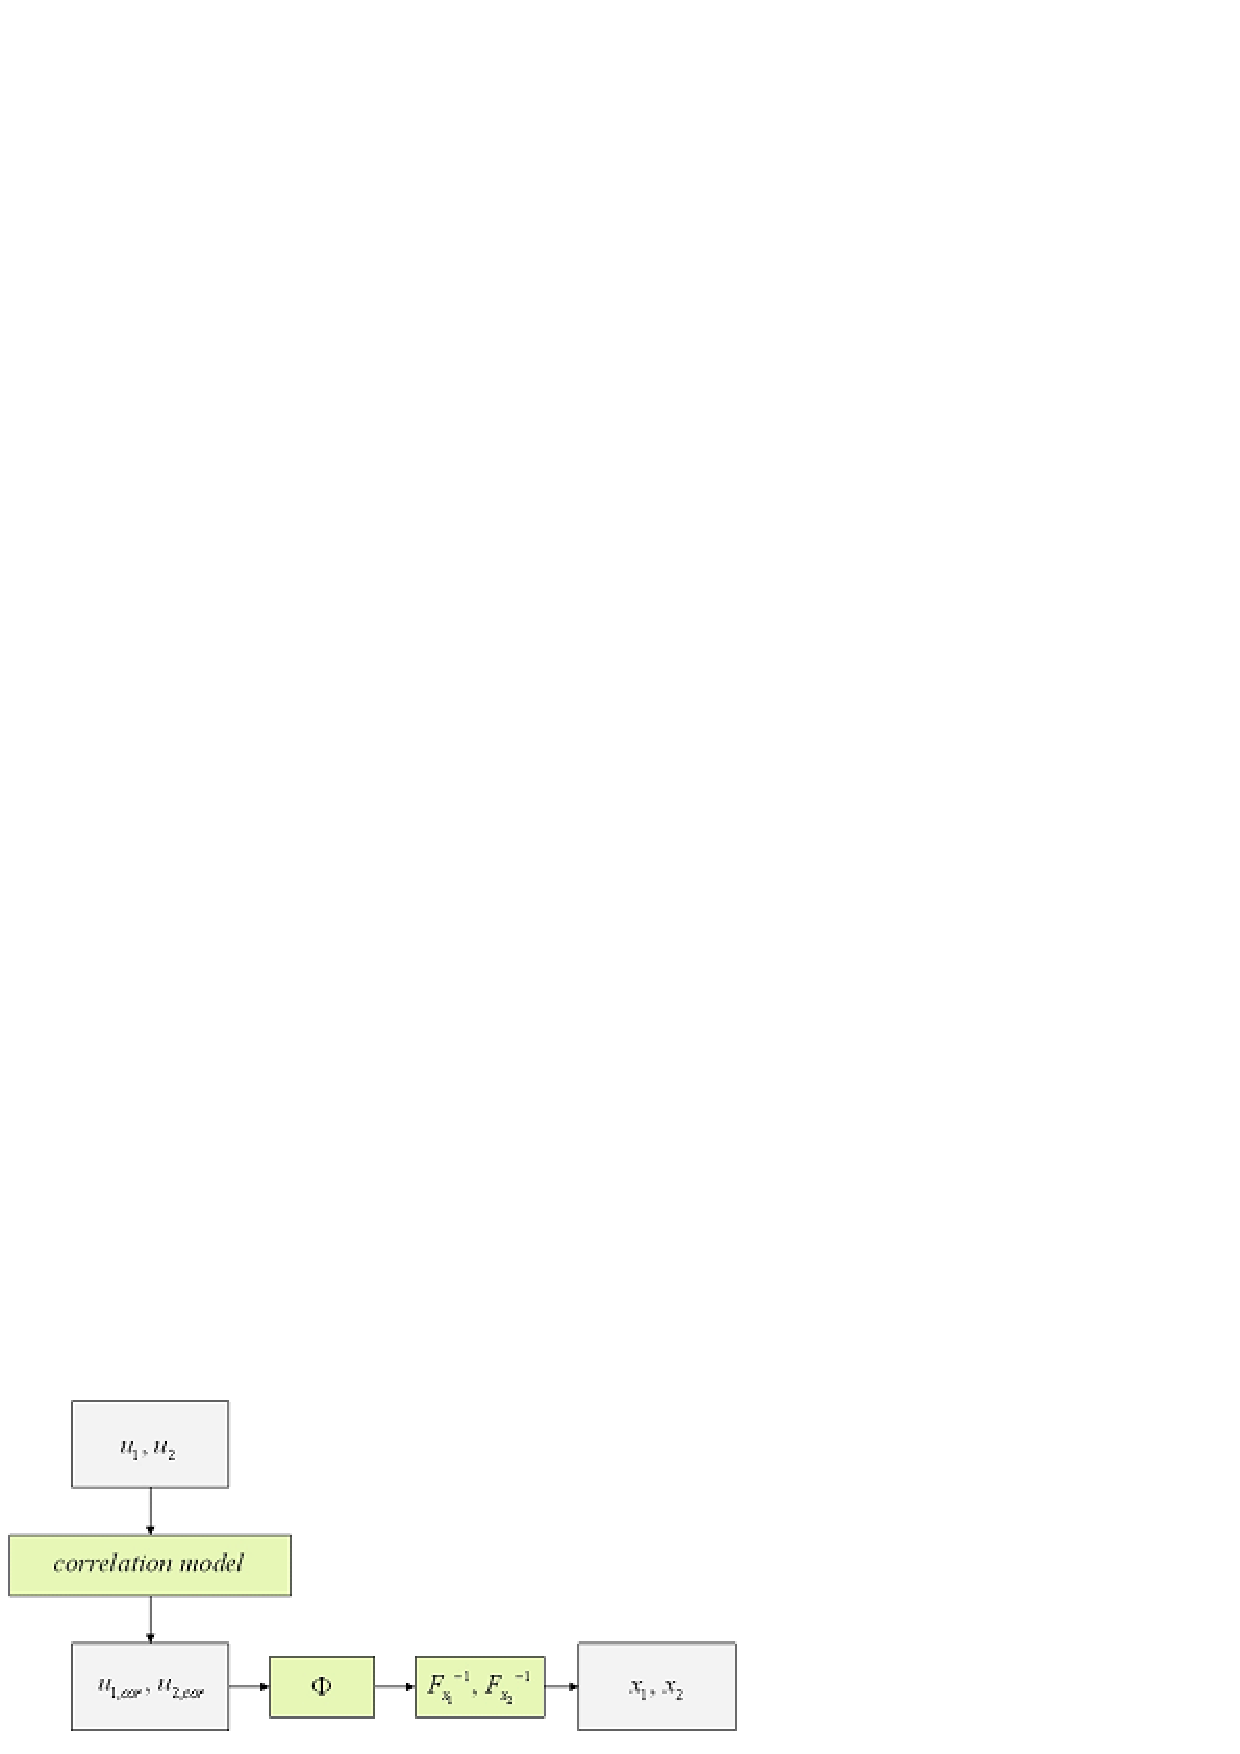
\includegraphics[width=1.0\columnwidth]{probabilisticLib_funcdesign_chapters/figloadmodels/image59.png}
\caption{Procedure for determining a load variable associated with randomly selected standard normally distributed variables for the case of correlated variables.}\label{fig:Figure_3.8}
\end{figure}

Since $U_{1,cor}$ and $U_{2,cor}$ are correlated variables, $X_1$ and $X_2$ are also correlated. Furthermore, since $U_{1,cor}$ and $U_{2,cor}$ are standard normally distributed and the translation from $U_{1,cor}$ and $U_{2,cor}$ to $X_1$ and $X_2$ is done in the exact same way as described in \Aref{Section_3.3}, it is automatically taken care of that $X_1$ and $X_2$ are distributed according to their prescribed distribution functions $F_{X_1}$ and $F_{X_2}$. The remainder of this section therefore focuses on the first part of the procedure: the generation of samples $u_{1,cor}$ and $u_{2,cor}$ of correlated variables $U_{1,cor}$ and $U_{2,cor}$.

The generation of $U_{1,cor}$ and $U_{2,cor}$ starts with the generation of realizations $u_1$ and $u_2$ of independent standard normally distributed random variables $U_1$ and $U_2$. Subsequently, $u_1$ is transformed into a sample $v$ of variable $V$ with distribution function $F_V(v)$. The transformation is done in similar style as explained in section \Aref{Section_3.3}, i.e. by making sure the probability of (non-)exceedance of $u_1$ and $v$ are equal: 
\begin{equation}
\Phi \left(u_{1} \right)=F_{V} \left(v\right)\Rightarrow v=F_{V} ^{-1} \left(\Phi \left(u_{1} \right)\right)\label{3.16)} 
\end{equation}

The $\Phi$ in this equation is the standard normal cumulative distribution function and $F_V(v)$ can be any cumulative distribution function, such as the normal, uniform or exponential distribution distribution. Subsequently, a sample $w$ is introduced that is dependent on $v$ and on a sample $u_2$ from a second standard normally distributed variable $U_2$:
\begin{equation} 
w=G\left(v,u_{2} \right)\label{ZEqnNum327839}
\end{equation}

The $G$ in this equation is a function that determines the correlation between $v$ and $w$. Subsequently, $v$ and $w$ are transformed back into samples $u_{1,cor}$ and $u_{2,cor}$ of standard normally distributed variables $U_{1,cor}$ and $U_{2,cor}$ by using the inverse CDFs or probabilities of (non-)exceedance. This leads to a $u_{1,cor}$ that identical to $u_1$, but $u_{2,cor}$ will be different from $u_2$ because of the use of the correlation function $G$. 

\begin{figure}[H]\centering
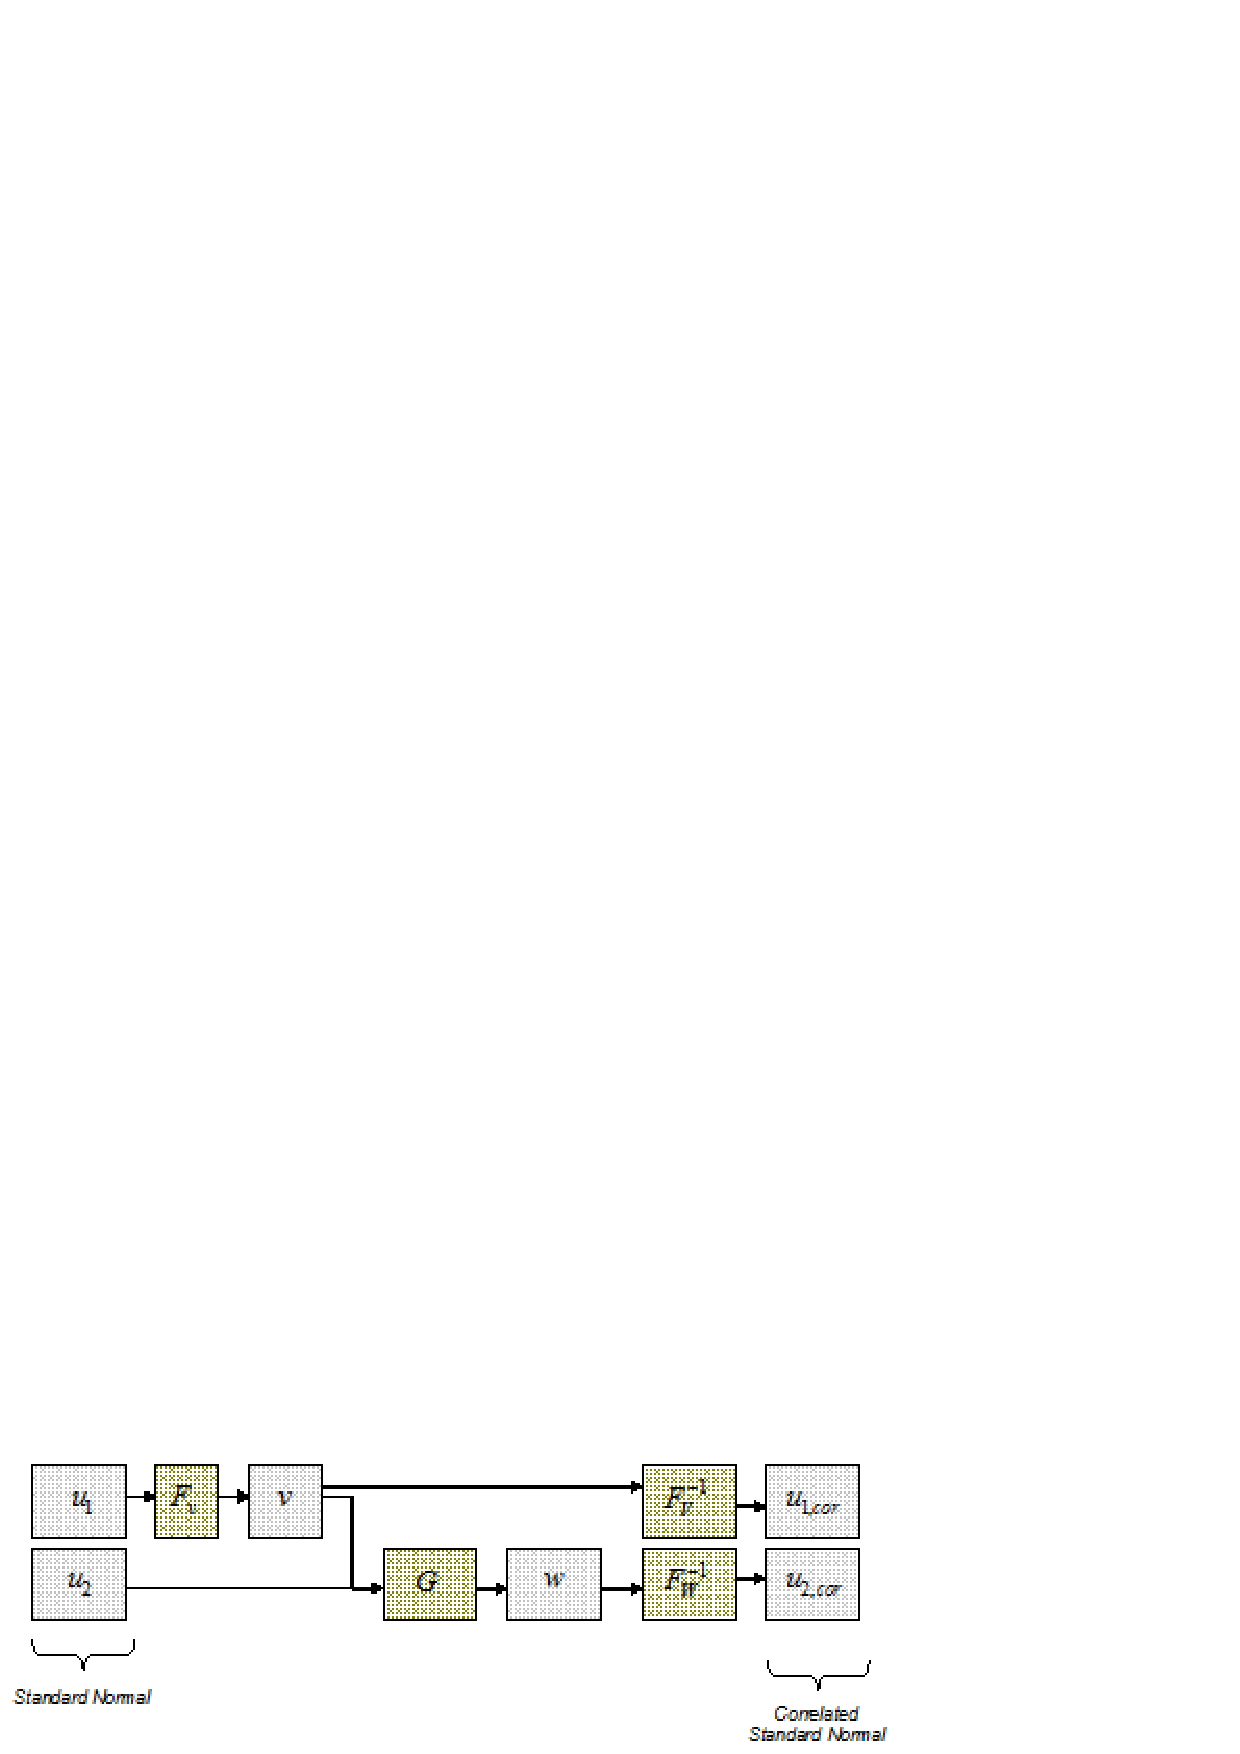
\includegraphics[width=1.0\columnwidth]{probabilisticLib_funcdesign_chapters/figloadmodels/image60.png}
\caption{Procedure for samples $u_{1,cor}$ and $u_{2,cor}$ of correlated standard uniform random variables $U_{1,cor}$ and $U_{2,cor}$.}\label{fig:Figure_3.9}
\end{figure}

The function $G$ is essentially the correlation model for variables $X_1$ and $X_2$. Many different functions $G$ can be used (note: $G$ is not a distribution function), also because the subsequent transformations $F_{V}^{-1}$ guarantee that $X_1$ and $X_2$ are distributed according to the pre-defined distribution functions $F_{X_1}$ and $F_{X_2}$. 
Naturally, function $G$ should be chosen such that it reproduces the observed correlation between variables $X_1$ and $X_2$ as well as possible. For a more detailed background on the derivation and application of correlation models in flood risk analysis, the interested reader is referred to the paper of \cite{Diermanse_Geerse_2012}. 

\section{Correlation models}\label{Section_3.4.2}

The following bi-variate correlation models are addressed in this section:
\begin{itemize}
\item Complete correlation,
\item PCR correlation model,
\item Volker correlation model,
\item HES correlation model,
\item Gaussian correlation model.
\end{itemize}
The complete correlation model is trivial as in this model $u_{2,cor}=u_{1,cor}=u_{1}$, this model will not be described any further. 

The PCR model is related to the Heteroscedastic (HES) model. Therefore a description of the PCR model in \Aref{Section_3.4.2.2} is preceded by a description of the HES model in \Aref{Section_3.4.2.3}. 

The Volker model is used to describe the wind-sea water level statistics in the tidal river areas. For a description of the Volker model, the reader is referred to \cite{basistochasten2017}. 

The bi-variate Gaussian correlation model has been implemented for practical purposes and it is described in \Aref{Gaussian_correlation_model}. The correlation model is a special case of the Gaussian copula model: the Gaussian copula model with $2$ variables gives the same results as the bi-variate Gaussian correlation model. The Gaussian copula model for $\geq 2$ random variables is described in \Aref{Gaussian_copula_model}. 

\subsection{HES correlation model}\label{Section_3.4.2.2}
The HES model is shorthand for ''Heteroscedastic model'', which means that the correlation varies depending on the values of $X_1$ and $X_2$. The model is very flexible and allows the user to set up a broad range of correlation structures. The model is described in the paper of \cite{Diermanse_Geerse_2012} and it is also referred to as the 'NL-model'.

The model describes the correlation between two random variables, $X_1$ and $X_2$ derived from two standard normal random variables $U_1$ and $U_2$. In the model, $U_1$ is the independent variable and $U_2$ the dependent variable (see \Fref{fig:Figure_3.9} for reference). 

The first step in the model is to transform the independent variable, $U_1$, sample $u_1$, into a standard exponentially distributed variable $V$, realization $v$.
\begin{equation} 
v=F_{V} ^{-1} \left(\Phi \left(u_{1} \right)\right)=-\ln \left(1-\Phi \left(u_{1} \right)\right)\label{ZEqnNum667656}
\end{equation}

The transformation is such that $v$ and $u_1$ have the same probability of (non-)exceedance (see \Aref{Section_2.2.3} for more information on this type of transformations). 

The next step is to compute the realization, $w$, of the dependent variable $W$. To describe the computation of $w$, first a couple of definitions are given. Let $\lambda (t)$ be a probability density function with a mean of $0$ and a standard deviation of $1$. This can be, but does not necessarily need to be, a standard normal density function. From $\lambda (t)$, distributions of the same type, but with different standard deviations, can be derived through the following transformation:
\begin{equation}
\lambda _{\sigma } \left(t\right)=\frac{1}{\sigma } \lambda \left({t\mathord{\left/ {\vphantom {t \sigma }} \right. \kern-\nulldelimiterspace} \sigma } \right)\label{3.19)}
\end{equation}

Density function $\lambda_{\sigma} (t)$ has a mean of $0$ and a standard deviation equal to $\sigma $. The cumulative distribution function, $\Lambda_{\sigma}$, is:
\begin{equation} 
\Lambda _{\sigma } \left(t\right)=\Lambda \left({t\mathord{\left/ {\vphantom {t \sigma }} \right. \kern-\nulldelimiterspace} \sigma } \right) \label{3.20)}
\end{equation}

The value of $w$ is computed as a combination of the realization $v$ of independent variable $V$ (correlated part) and of the realization $u_2$ of the standard normal variable $U_2$ (uncorrelated part):
\begin{equation}
w=v+\delta +\Lambda _{\sigma \left(v \right)}^{-1} \left(\Phi \left(u_{2} \right)\right)\label{ZEqnNum481579}
\end{equation}

Where $\delta$ is an offset that can be chosen arbitrarily and $\Lambda_{\sigma \left(v \right)}^{-1}$ is the inverse of the CDF of the uncorrelated part, with a $\sigma$ that can depend on the value of $v$. 
The right hand side of this equation is essentially the description of function $G$ of formula \eqref{ZEqnNum327839}, see \Fref{fig:Figure_3.9}. A schematic graph of the relationship between $w$ and $v$ is shown in \Fref{fig:Figure_3.10}. The dashed line shows the correlated part of the relationship between $v$ and $w$. The distribution around that line, in this case a normal distribution, is shown for two values of $v$. Note that in \Fref{fig:Figure_3.10} the standard deviation can vary with $v$. That is, for increasing values of $v$, the standard deviation of $w$ values around $v$ can increase or decrease. 
For a constant variance of $w$ for all $v$, $\sigma (v)$ is simply set constant. The relationship $\sigma (v)$ needs to be determined a-priori and included as input in the correlation model. The procedure to determine $\sigma (v)$ is an iterative one, and is described in \cite{Diermanse_Geerse_2012}. 

\Note{when $\Lambda _{\sigma(v)}$ is normally distributed with constant standard deviation $\sigma(v)=\sigma>0$, then equation \eqref{ZEqnNum481579} simplifies to $w=v+\delta+\sigma u_{2}$. This special case of the HES model is called the Constant Spread (CS) correlation model.}

\begin{figure}[H]\centering
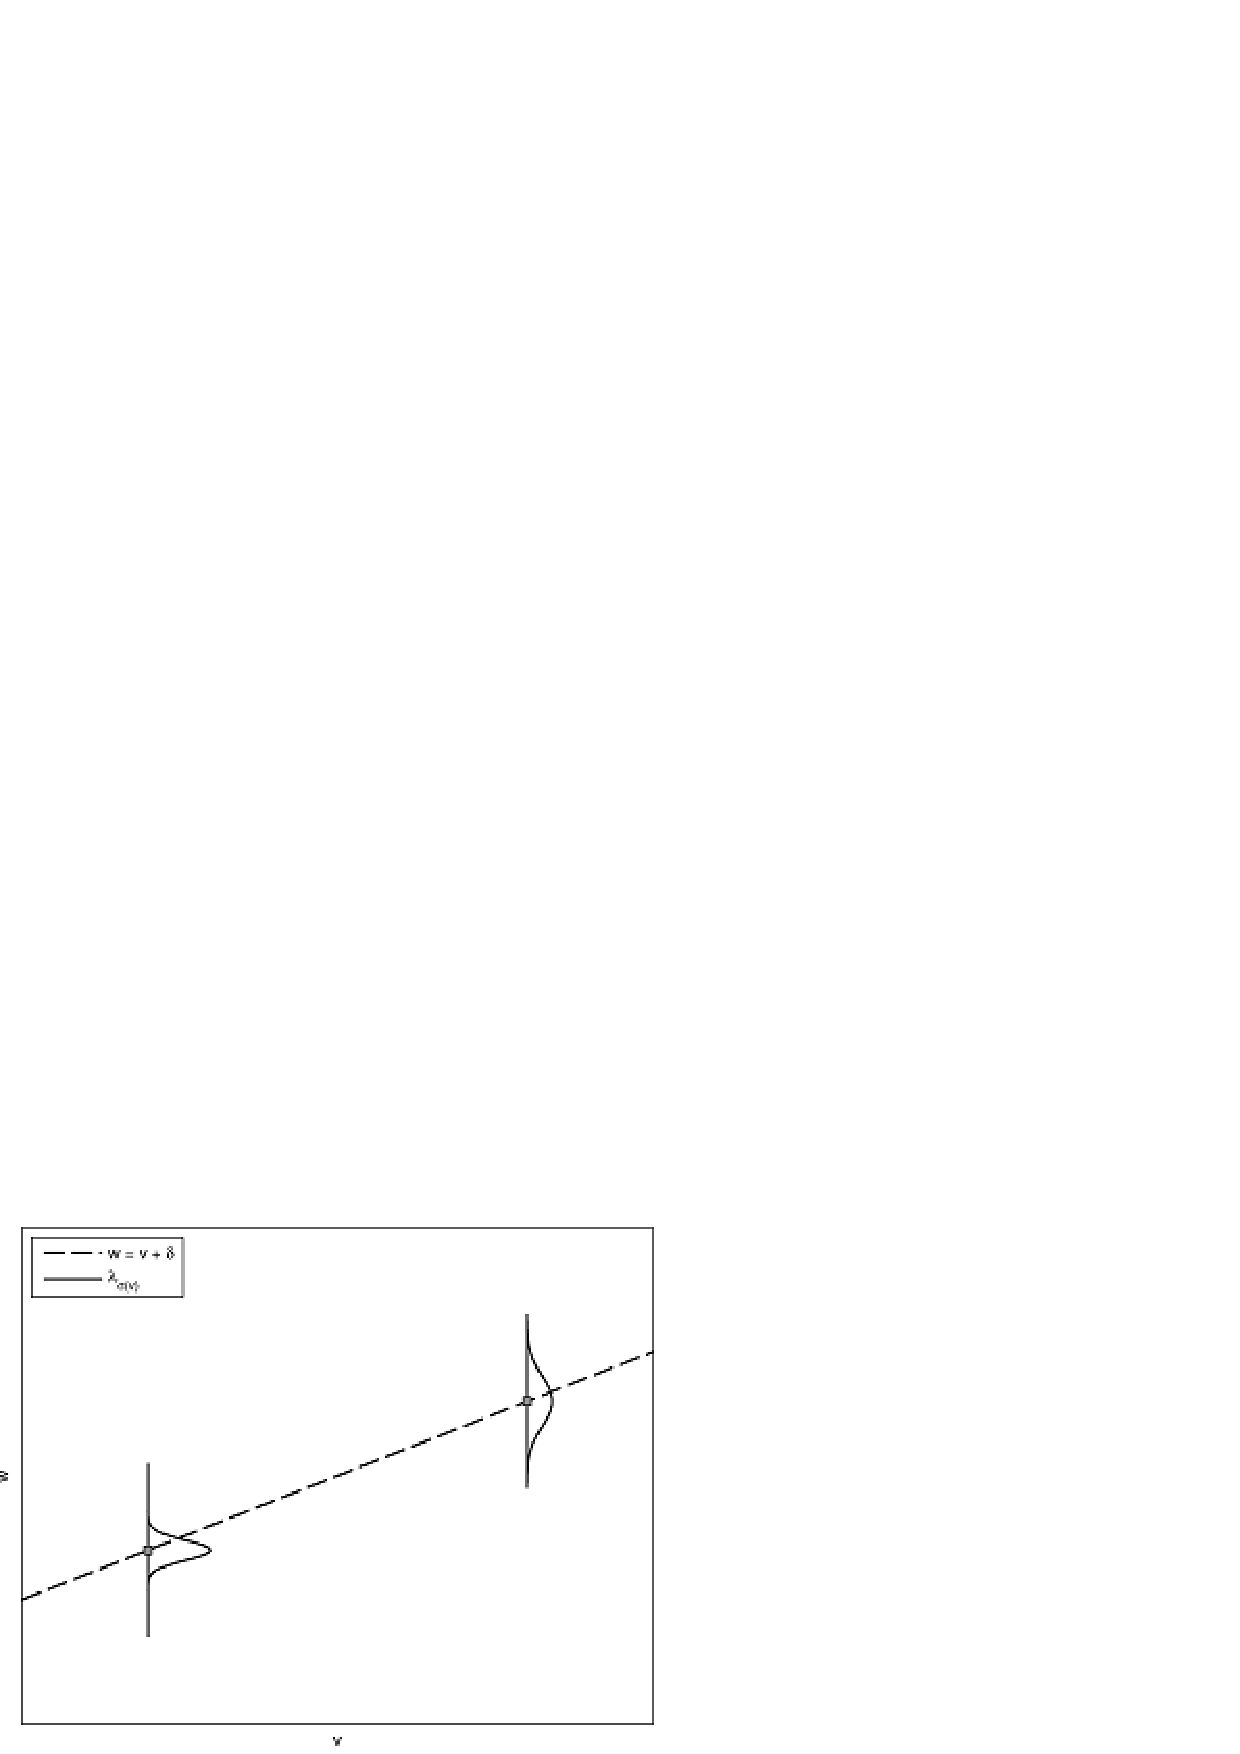
\includegraphics[width=0.8\columnwidth]{probabilisticLib_funcdesign_chapters/figloadmodels/image61.png}
\caption{Schematic illustrating the relationship between $w$, $v$, and $u_2$ in the NL model.}\label{fig:Figure_3.10}
\end{figure}

The next step in the correlation model is to transform the variables $V$ and $W$ back to standard normal variables $U_{1,cor}$ and $U_{2,cor}$. For this purpose, the distribution functions $F_V(v)$ and $F_W(w)$ are required. 
The transformation from $V$ to $U_{1,cor}$ is done as follows:
\begin{equation}
u_{1,cor} =\Phi ^{-1} \left(F_{V} \left(v\right)\right)=\Phi ^{-1} \left(1-e^{-v} \right)\label{3.22)}
\end{equation}

This transformation is the inverse of the transformation in equation \eqref{ZEqnNum667656}. This leads to a $u_{1,cor}$ that is exactly the same as $u_1$. 

The transformation from $W$ to $U_{2,cor}$ is done as follows:
\begin{equation} 
u_{2,cor} =\Phi ^{-1} \left(F_{W} \left(w\right)\right)\label{ZEqnNum307043} 
\end{equation}

This is generally less straightforward because there is often no analytical description available of the distribution function $F_W(w)$. The distribution can be derived from the following integral (according to the theorem of total probability):
\begin{equation} 
F_{w} \left(w\right)=\int _{0}^{\infty }f_{V} \left(v\right)P\left[W<w\left|v\right. \right]dv= \int _{0}^{\infty }\exp \left(-v\right)\Lambda _{\sigma \left(v\right)} \left(w-v-\delta \right)dv \label{ZEqnNum141107}
\end{equation}

\subsection{PCR correlation model}\label{Section_3.4.2.3}
The correlation model referred to as PCR (PC-Ring) is given this naming convention because it is the correlation model which was developed and used as the standard correlation model in PC-Ring. The model is similar to the HES, except that it includes a simplifying approximation for reasons of computational efficiency. The assumption is that variable $W$ is exponentially distributed, which means that the transformation \eqref{ZEqnNum307043} can be done without the numerical integration of equation \eqref{ZEqnNum141107} . The reduction in computation time was valuable in the period that PC-Ring was developed. 

Just as the HES model, the PCR model has an independent variable $V$ and a dependent variable $W$. $V$ is once again standard exponentially distributed and the realizations $v$ of this variable can be derived using equation \eqref{ZEqnNum667656}. 

Realizations of variable $W$ are derived using equation \eqref{ZEqnNum481579}. However, because of the assumption of exponentially distributed $W$, the parameter $\delta$ and function $\Lambda$ are given by:
\begin{equation}
\delta=-\frac{\sigma ^{2} }{2}
\end{equation}
and 
\begin{equation}
\Lambda _{\sigma \left(v \right)}^{-1} \left(\Phi \left(u_{2} \right)\right) = \sigma u_{2} 
\end{equation}
So:
\begin{equation}
w=v-\frac{\sigma ^{2} }{2} +\sigma u_{2} \label{ZEqnNum466239}
\end{equation}

In the PCR model, parameter $\sigma$ determines the measure of correlation. Small values of $\sigma$ correspond to a strong correlation, whereas large values of $\sigma$ correspond to weak correlation. 

\Fref{fig:Figure_3.11} shows the assumed probability density function of variable $W$ in the PCR model, i.e the standard exponential density function. Furthermore, it shows the probability density function of the HES model, $f_W(w)$, in case of a constant standard deviation. As can be seen, $f_W(w)$ converges to the standard exponential density function in the right tail. In other words: for larger values of $w$, variable $W$ of the HES model with constant correlation is (asymptotically) standard exponentially distributed. 

As mentioned, the PCR model assumes that the variable $W$ is standard exponentially distributed over the entire domain. This means the transformation from variable $W$ to the standard normal variable $U_{2,cor}$ is done by:
\begin{equation} 
u_{2,cor} =\Phi ^{-1} \left(F_{W} \left(w\right)\right)=\Phi ^{-1} \left(1-e^{-w} \right)\label{ZEqnNum122862}
\end{equation}

Since equation \eqref{ZEqnNum122862} is much easier to solve than equations \eqref{ZEqnNum141107} and \eqref{ZEqnNum307043}, the PCR-model requires less computation time than the HES model. However, by making the assumption of a standard exponential distribution function, the PCR-model introduces an error for small $w$, as can be seen in \Fref{fig:Figure_3.11}. This error will propagate in the value of $u_{2,cor}$ and eventually also in $x_2$, i.e. the realization of the associated ''real-world'' variable $X_2$. The reason why the assumption of the PCR model is reasonable is that for failure computations only large values of load variables are relevant and the error introduced by the assumption is generally negligible. 

\Note{this assumption can become less sound when smaller values of the load variables are relevant for failure as well. For instance at a location near the sea in a tidal river system, failure (flooding) most likely occurs during an event with extremely high sea water levels in combination with ''average'' river discharges. If the river discharge is estimated from the PCR model, errors may be introduced in estimating the probability of occurrence of such an event. However an analysis of the consequences has shown the practical effects on calculated water levels are marginal.

\begin{figure}[H]\centering
\includegraphics*[width=4.16in, height=3.27in, keepaspectratio=false]{probabilisticLib_funcdesign_chapters/figloadmodels/image62.png}
\caption{Probability density function of variable $W$ in the PCR-model, compared with the density function of a standard exponential distribution function.}\label{fig:Figure_3.11}
\end{figure}

\subsection{Gaussian correlation model}\label{Gaussian_correlation_model}
This section describes the bi-variate Gaussian correlation model that can be used to describe a simple correlation between standard normal random variables.
Given is the following correlation matrix $C$ with correlation coefficient $\rho\in[-1,1]$:
\begin{equation} 
C = \begin{bmatrix}
1.0 & \rho\\
\rho & 1.0\\
\end{bmatrix}
\end{equation} 

The 'lower' Cholesky decomposition of this matrix is (i.e. $P\times P^{T}=C$):
\begin{equation} 
P = \begin{bmatrix}
1.0 & 0.0\\
\rho & \sqrt{1-\rho^2}\\
\end{bmatrix}
\end{equation} 

Given an uncorrelated sample of standard normal random variables $u_1$ and $u_2$, the correlated sample $u_{1,cor}$ and $u_{2,cor}$ is derived as follows:
\begin{equation} 
[u_{1,cor},u_{2,cor}]=[u_1,u_2]\times P^{T} = [u_1,u_2]\times
\begin{bmatrix}
1.0 & \rho\\
0.0 & \sqrt{1-\rho^2}\\
\end{bmatrix}
\end{equation} 

This simplifies to:
\begin{equation} 
u_{1,cor}=u_1
\end{equation} 
and
\begin{equation} 
u_{2,cor}=u_1\rho+u_2\sqrt{1-\rho^2}
\end{equation}

The following figure pictures the uncorrelated and correlated samples for $\rho=0.5$.

\begin{figure}[H]\centering
\includegraphics*[width=4.16in, height=3.27in, keepaspectratio=false]{probabilisticLib_funcdesign_chapters/figsystemreliability/fig_gaussian_model.png}
\caption{Uncorrelated (left) and correlated (right) samples according to the Gaussian correlation model assuming $\rho=0.5$.}
\end{figure}

Furthermore, the following holds:
\begin{itemize}
\item When $\rho=0.0$ then the correlated sample is equal to the uncorrelated sample.
\item When $\rho=1.0$ then $u_{2,cor} = u_1$ (complete correlation).
\item When $\rho=-1.0$ then $u_{2,cor} = -u_1$ (reverse complete correlation).
\end{itemize}

\subsection{Gaussian copula model}\label{Gaussian_copula_model}
This section presents a Gaussian copula model, which can be used to describe correlation between $\geq 2$ variables in the $U$-space. The correlation coefficients are in this case stored in a correlation matrix.

A correlation matrix is a table showing correlation coefficients (i.e. product moment correlations) between variables. The diagonal of the table is always a set of ones, because the correlation between a variable and itself is always $1.0$. The matrix is also symmetric -- the correlation coefficient between variables $X$ and $Y$ is equal to the correlation coefficient between variables $Y$ and $X$. Moreover, the matrix must be positive definite, that is:
\begin{equation}
x^T\cdot C\cdot x>0 \mbox{ for all $x\in\Re^{n}\setminus\{0\}$ }
\end{equation}
where $C$ is a correlation matrix with size $n\times n$ and $T$ denotes the transpose.

In the \probLib, it is possible to describe correlations between random variables in a correlation matrix. The procedure to generate correlated samples $u_{cor}$ is as follows (see \cite{Diermanse_etal_2014}):
\begin{enumerate}
\item Derive a matrix $P$ for which $P\cdot P^{T}=C$ through Cholesky decomposition of correlation matrix $C$ with size $n\times n$ (see \cite{Strang_1982}).
\item Sample values $u_1,...,u_n$ from the standard normal distribution function and store the values in a $1\times n$ vector $u$.
\item The sample of the correlated standard normally distributed random variables $u_{cor}$ is then defined as follows: $u_{cor}=u\cdot P^{T}$.
\end{enumerate}

In the \probLib a special care is taken of correlation matrices with off-diagonal $\pm1.0$ elements. Such matrices usually do not satisfy the positive definite requirement. In order to perform calculations with such matrices, a two-step procedure is applied, during which the original matrix is decomposed into two matrices: (1) a matrix without the off-diagonal $\pm1.0$ elements and (2) a matrix with $0.0$ and $\pm1.0$ entries that indicate the positions of the off-diagonal $\pm1.0$ elements in the original matrix. The Cholesky decomposition is performed on the first matrix, highly increasing the chance that the positive definite requirement will be satisfied. The vector $u$ is first multiplied with the Cholesky decomposition matrix entailing a correlated sample without the full correlation cases. The resulting sample vector is then multiplied by the second matrix assuring that the same values are assigned to the fully correlated variables. The procedure is explained in more detail in the following example.

Consider the following correlation matrix $C$ with $\rho_{1,2}=\rho_{2,1}=1.0$:
\begin{equation} 
C = \begin{bmatrix}
1.0 & \rho_{1,2} & ... & \rho_{1,j} & ... & \rho_{1,n}\\
\rho_{2,1} & 1.0 & ... & \rho_{2,j} & ... &  \rho_{2,n}\\
... & ... & ... & ... & ...  & ...\\
\rho_{i,1} & \rho_{i,2} & ... & 1.0 & ... & \rho_{i,n}\\
... & ... & ... & ... & ...  & ...\\
\rho_{n,1} & \rho_{n,2} & ... & \rho_{n,j} & ... & 1.0\\
\end{bmatrix}
\end{equation} 

Matrix $C$ is decomposed into matrix $C_1$ and $C_2$. Matrix $C=C_1$ except for off-diagonal values found in the second row and column. These values are all equal to $0.0$. Matrix $C_2$ is an identity matrix except for the second row and column where $\rho_{2,1}=1.0$, $\rho_{i,2}=0.0$ for $i=1...n$ and $\rho_{2,j}=0.0$ for $j=2...n$. 
\begin{equation} 
C_1 = \begin{bmatrix}
1.0 & \mathbf{0.0} & ... & \rho_{1,j} & ... & \rho_{1,n}\\
\mathbf{0.0} & \mathbf{1.0} & ... & \mathbf{0.0} & ... &  \mathbf{0.0}\\
... & ... & ... & ... & ...  & ...\\
\rho_{i,1} & \mathbf{0.0} & ... & 1.0 & ... & \rho_{i,n}\\
... & ... & ... & ... & ...  & ...\\
\rho_{n,1} & \mathbf{0.0} & ... & \rho_{n,j} & ... & 1.0\\
\end{bmatrix}
\end{equation} 

\begin{equation} 
C_2 = \begin{bmatrix}
1.0 & \mathbf{0.0} & ... & 0.0 & ... & 0.0\\
\mathbf{1.0} & \mathbf{0.0} & ... & \mathbf{0.0} & ... &  \mathbf{0.0}\\
... & ... & ... & ... & ...  & ...\\
0.0 & \mathbf{0.0} & ... & 1.0 & ... & 0.0\\
... & ... & ... & ... & ...  & ...\\
0.0 & \mathbf{0.0} & ... & 0.0 & ... & 1.0\\
\end{bmatrix}
\end{equation} 

Assuming that $P$ is the Cholesky decomposition of matrix $C_1$, then the correlated sample $u_{cor}$ is derived as follows: 
\begin{equation} 
u_{cor}=u\cdot P^{T}\cdot C_2^{T}
\end{equation} 
\include{funcdesign_chapters/appConversions}
\include{common/glossary}

\end{document}
